%-----------------------------------------------------------------------
% Beginning of article-template.tex
%-----------------------------------------------------------------------
%
%    This is a template file for proceedings articles prepared with AMS
%    author packages, for use with AMS-LaTeX.
%
%    Templates for various common text, math and figure elements are
%    given following the \end{document} line.
%
%%%%%%%%%%%%%%%%%%%%%%%%%%%%%%%%%%%%%%%%%%%%%%%%%%%%%%%%%%%%%%%%%%%%%%%%

%    Remove any commented or uncommented macros you do not use.

%    Replace amsproc by the name of the author package.
\documentclass{amsproc}

%    If you need symbols beyond the basic set, uncomment this command.
%\usepackage{amssymb}

%    If your article includes graphics, uncomment this command.
%\usepackage{graphicx}

%    If the article includes commutative diagrams, ...
%\usepackage[cmtip,all]{xy}

%    Include other referenced packages here.
\usepackage{}


\usepackage{amssymb}
\usepackage{graphicx}
\usepackage{amsmath}

%    Update the information and uncomment if AMS is not the copyright
%    holder.
%\copyrightinfo{2009}{American Mathematical Society}


\newcommand{\be}{\begin{equation}}
\newcommand{\ee}{\end{equation}}

\newcommand{\ben}{\begin{equation*}}
\newcommand{\een}{\end{equation*}}

\newcommand{\ba}{\begin{align}}
\newcommand{\ea}{\end{align}}

\newcommand{\ban}{\begin{align*}}
\newcommand{\ean}{\end{align*}}

\newcommand{\df}{\; \mathrm{d}}




\usepackage{color}
\definecolor{darkblue}{rgb}{0,0,0.5}
\definecolor{darkred}{rgb}{0.5,0,0}
\definecolor{darkgreen}{rgb}{0,0.5,0}
\definecolor{orange}{rgb}{0.9,0.58,0}

\newcommand{\at}[1]{\textbf{\textcolor{orange}{(#1 --at)}}}

\newtheorem{theorem}{Theorem}[section]
\newtheorem{lemma}[theorem]{Lemma}

\theoremstyle{definition}
\newtheorem{definition}[theorem]{Definition}
\newtheorem{example}[theorem]{Example}
\newtheorem{xca}[theorem]{Exercise}

\theoremstyle{remark}
\newtheorem{remark}[theorem]{Remark}

\numberwithin{equation}{section}

\begin{document}

% \title[short text for running head]{full title}
\title{Roots of the Zeta Function, Random Matrices and Quantum Mechanics}

%    Only \author and \address are required; other information is
%    optional.  Remove any unused author tags.

%    author one information
% \author[short version for running head]{name for top of paper}
\author{Aashish Tripathee}
\address{}
\curraddr{}
\email{aashisht@mit.edu}
\thanks{}




%    The 2010 edition of the Mathematics Subject Classification is
%    now available.  If you are citing a classification from the
%    new scheme, use the following input coding instead.
%\subjclass[2010]{Primary }

\date{}

\begin{abstract}
In this paper, we explore three different algorithms to numerically calculate the non-trivial zeros of the Riemann Zeta function, $\zeta(t)$, namely, the Euler-Maclaurin method, alternating series method and the Riemann-Siegel formula. We then introduce random matrices and investigate any possible connection between their eigenvalues and the non-trivial zeros of $\zeta(t)$. We introduce the Hilbert-Polya conjecture as an alternate approach to proving the Riemann hypotheis. We investigate some of the properties of the eigenvalues of the Berry-Keating Hamiltonian.
\end{abstract}



\maketitle



%%%%%%%%%%%%%%%%%%%%%%%%%%%%%%%%%%%%%%%%%%%%%%%%%%%%%%%%%%%%%%%%%%%%%%%%

%    Templates for common elements of an article; for additional
%    information, see the AMS-LaTeX instructions manual, instr-l.pdf,
%    included in every AMS author package, and the amsthm user's guide,
%    linked from http://www.ams.org/tex/amslatex.html .

%    Section headings

\section{The Riemann Zeta Function}
The Riemann Zeta function is a function of a complex variable $s$, that analytically continues the sum of the infinite series,
\be
\zeta(s) = \sum_{n = 1}^{\infty} \frac{1}{n^2} \;.
\ee
$\zeta(s)$ converges for $\mathrm{Re}(s) > 1$, so we will restrict ourself to that domain for this paper. The Zeta function was first studied by Euler in 1740 but his study was limited to real, positive, integer values of $s$ only. Riemann later extended the function to complex valued $s$ in his 1859 paper ``On the Number of Primes Less Than a Given Magnitude''. There are multiple ways of defining $\zeta(t)$. It can, for example, also be defined as the integral,
\be
\zeta(s) = \frac{1}{ \Gamma(s) } \int_0^{\infty} \frac{ x^{s -1} }{ e^x - 1} \df x \;,
\ee
where $\Gamma(s) = \int_0^{\infty} x^{s - 1} e^{-x} \df x$. A particularly important represntation of the zeta is using the Euler product formula, 
\be
\zeta(s) = \prod_{\mathrm{p~prime}} \frac{1}{1 - p^{-s}}
\ee
This form was proved by Euler in 1737 and is important, for example, because it can be used to prove that there are infinitely many primes. Consider the case when $s = 1$. Then,
\begin{align*}
 1 &= \zeta(1) \left( 1 - \frac{1}{2} \right) \left( 1 - \frac{1}{3} \right) \left( 1 - \frac{1}{5} \right) \left( 1 - \frac{1}{7} \right) \ldots \\
 1 &= \zeta(1) \frac{1}{2} \cdot \frac{2}{3} \cdot \frac{4}{5} \cdot \frac{6}{7} \ldots \\
  1 &= \zeta(1) \frac{1 \cdot 2 \cdot 4 \cdot 6 \ldots}{2 \cdot 3 \cdot 5 \cdot 7 \ldots } 
\end{align*}
But, $\zeta(1) = 1 + \frac{1}{2} + \frac{1}{3} + \frac{1}{4} + \frac{1}{5} + \frac{1}{7} + \ldots$, which gives,
\begin{equation*}
 1 + \frac{1}{2} + \frac{1}{3} + \frac{1}{4} + \frac{1}{5} + \frac{1}{7} + \ldots =  \frac{2 \cdot 3 \cdot 5 \cdot 7 \ldots }{1 \cdot 2 \cdot 4 \cdot 6 \ldots}
\end{equation*}
But the left hand side of this equation diverges, which means the numerator in the right hand side diverges too, which means there must be infinitely many primes.  

Another important form of the zeta function is the functional equation, written as,
\be
\zeta(s) = 2^s \pi^{s - 1} \sin{ \left( \frac{\pi s}{2} \right) } \Gamma(1 - s) \zeta( 1 - s) \;.
\ee

\section{Numerical Determination of the Roots of the Zeta Function}
\subsection{Euler-Maclaurin Formula}
The Euler-Maclaurin formula is a very popular tool used in numerical analysis as a connection between integrals and sums. It can be used to reformulate an integral as a sum or vice versa and is very popular in analytical number theory where it is used to compute sums in terms of integrals. The formula was developed in the early eighteenth century and came as a result of trying to extend the sum $\sum_{k} n^k$ for $k$'s other than 1. It was developed independently by Leonhard Euler and Colin Maclaurin around 1735- Euler to extend the sum just mentuoned and Maclaurin to compute integrals. The formula can be written as,

\begin{align}
\sum_{n = M}^{N} f(n) = &\int_M^N f(x) \df x + \frac{1}{2} \left[ f(N) - f(M) \right] + \\
&\sum_{j = 1}^{\nu} \frac{B_{2j}}{ (2j)! } \left[ f^{( 2j - 1)}(N) - f^{(2j - 1)} (M) \right] + R
\end{align}

The remainder $R$ is given by, 
\be 
R_{2 \nu} = - \frac{ s (s + 1) \ldots (s + 2 \nu) }{ (2 \nu + 1)! } \int_N^{\infty} B_{2 \nu + 1}(x) x^{-s - 2\nu - 1} \df x \;.
\ee
It can be shown that R satisfies the inequality \cite{},
\be
\left| R_{2 \nu - 2} \right| \le \left| \frac{s + 2 \nu - 1}{ \mathrm{Re}(s) + 2\nu - 1 } \right|  \cdot \left| B_{2 \nu} \right| \;.
\ee
This means, if $B_{2 \nu}$ is the first term we ignore in our sum, the remainder will be at most $\left| \frac{s + 2 \nu - 1}{ \sigma + 2\nu - 1 } \right|  \cdot \left| B_{2 \nu} \right|$. 

If we apply the Euler-Maclaurin formula to $\zeta(s) = \sum_{1}^{\infty} n^{-s}$, $R$ will not be small enough to be ignored \cite{}. So, we instead apply the formula to the sum, $\sum_{N}^{\infty} n^{-s}$. Notice that,
\begin{align*}
 \sum_{n = 1}^{\infty} n^{-s} - \sum_{n = 1}^{N - 1} n^{-s} &= \sum_{N}^{\infty} n^{-s} \\
 \zeta(s) - \sum_{n = 1}^{N - 1} n^{-s} &= \sum_{N}^{\infty} n^{-s} 
\end{align*}

\be
\label{eqn:euler_main}
\zeta(s)  = \sum_{n = 1}^{N - 1} n^{-s} + \sum_{N}^{\infty} n^{-s} = \sum_{n = 1}^{N - 1} n^{-s} + \chi(s)
\ee

The first term is easy to compute and we can use the Euler-Maclaurin formula to compute $\chi(s)$. Applying the formula, 

\begin{align*}
\chi(s) &= \int_N^{\infty} x^{-s} \df x + \frac{1}{2} N^{-s} + \sum_{j = 1}^{\nu} \frac{B_{2j}}{ (2j)! } \left[ - (n^{-s})^{(2j - 1)} (N) \right] + R \\
& \approx \frac{1}{s - 1} N^{1 - s}  + \frac{1}{2} N^{-s} + \frac{B_2}{2} s N^{-s - 1} + \ldots + \left[ \frac{B_{2 \nu}}{ (2\nu)! } s(s + 1)  \ldots (s + 2 \nu - 2) N^{( -s - 2\nu + 1)} \right]
\end{align*}

The sum we need to calculate can be divided into four different parts, defined as follows:
\begin{align*}
 A &= \sum_{n = 1}^{N - 1} n^{-s} \\
 B &= \frac{1}{s - 1} N^{1 - s} \\
 C &= \frac{1}{2} N^{-s} \\
 D &= \frac{B_2}{2} s N^{-s - 1} + \ldots + \left[ \frac{B_{2 \nu}}{ (2\nu)! } s(s + 1)  \ldots (s + 2 \nu - 2) N^{( -s - 2\nu + 1)} \right]
\end{align*}
Then, 
\begin{equation*}
 \zeta(s) \approx A + B + C + D \;,
\end{equation*}
with the error at most $\left| \frac{s + 2 \nu - 1}{ \mathrm{Re}(s) + 2\nu - 1 } \right|  \cdot \left| B_{2 \nu} \right|$. 

This formula can be now used to compute $\zeta(s)$ and is very easy to implement. A sample implementation can be found in Section \ref{}. 

\subsection{Alternating Series (Dirichlet Eta Function)}
Consider the following sum:
\be
\label{eqn:alternating_series}
\eta(s) = \sum_{n = 1}^{\infty} \frac{ (-1)^{n - 1} }{n^s} = \frac{1}{1^s} - \frac{1}{2^s} + \frac{1}{3^s} - \frac{1}{4^s} + \ldots
\ee
Comparing this to,
\begin{equation*}
 \zeta(s) = \sum_{n = 1}^{\infty} n^{-s} = \frac{1}{1^s} + \frac{1}{2^s} + \frac{1}{3^s} + \frac{1}{4^s} + \ldots
\end{equation*}
it's clear that,
\be
\label{eqn:dir_zeta}
\eta(s) = \left( 1 - 2^{1 - s} \right) \zeta(s) \;.
\ee
$\eta(s)$ is called the Dirichlet eta function, sometimes also called the alternating zeta function as it's the same sum as zeta function except the sign of the terms alternates between + and -. 

Equation \ref{eqn:dir_zeta} means that if we can find a way to evaluate $\eta(s)$, we can evaluate $\zeta(s)$ using that. 

Consider using Euler's transformation of alternating series to the series defined in Equation \ref{eqn:alternating_series} to accelerate its convergence. Euler's transform of alternating series is defined as,
\be
\label{eqn:euler_transform}
\sum_{n = 0}^{\infty} (-1)^n a_n = \sum_{n = 0}^{\infty} (-1)^n a_0 \frac{ 1 }{2^{n + 1}} \Delta^n \;,
\ee
where $\Delta^n$ is the $n^{\mathrm{th}}$-order forward difference of the function $f(x)$ given by,
\begin{equation*}
 \Delta^n[f](x) = \sum_{k = 0}^{n} {n \choose k} (-1)^{n - k} f(x + k)
\end{equation*}
Comparing \ref{eqn:euler_transform} to $\eta(s) = \sum_{n = 1}^{\infty} \frac{ (-1)^{n - 1} }{n^s} = \sum_{n = 0}^{\infty} \frac{ (-1)^n }{ (n + 1)^s }$, it is clear that,
\begin{align*}
\eta(s) &= \sum_{n=0}^{\infty} (-1)^n 1^{-s} \frac{1}{ 2^{n + 1} } \Delta^n \\
        &= \sum_{n=0}^{\infty} (-1)^n 1^{-s} \frac{1}{ 2^{n + 1} } \sum_{k=0}^{n} {n \choose k} \frac{ (-1)^n }{ (-1)^k } \frac{1}{ (k + 1)^s } \\
        &= \sum_{n=0}^{\infty} \frac{1}{ 2^{n + 1} } \sum_{k=0}^{n} {n \choose k} \frac{ (-1)^k }{ (k + 1)^s }
\end{align*}
This sum converges much faster than the original sum as it is exponential in $n$ and so, is much more efficient. A Python implementation that calculates this sum and uses it to calculate the Zeta function can be found in Section. \ref{}. 

\subsection{Riemann-Siegel Formula}
We won't consider the derivation of the Riemann-Siegel formula here but the formula can be expressed as,
\be
Z(t) = 2 \sum_{n^2 < (t / 2 \pi )} n^{-1/2} \cos{ \left[ \theta(t) - t \log{n} \right] } + R \;,
\ee
with
\begin{equation}
 \theta(t) = \Gamma\left[ \frac{ 2 i t + 1}{4} \right] - t \frac{\log{\pi}}{2}
\end{equation}
\begin{align}
R = \frac{ e^{-i\nu(t)} e^{-t \pi / 2} }{ (2 \pi)^{1/2} (2 \pi)^{it} e^{-i t / 4} \left( 1 - i e^{-t \pi} \right) } \int_{C_N} \frac{ (-x)^{-(1/2) + i t}  e^{-Nx}}{ e^x - 1} \df x,
\end{align}
where $C_n$ is a contour which descends the real axis from $\infty$ to $(2 N + 1) \pi$, circles the boundary of the disk $\left| s \right| \le (2N + 1) \pi$ once and goes back to $\infty$ \ref{}.

The reaminder $R$ can be simplified and expressed in the following form. The details are in Edwards book.
\be
R \sim (-1)^{N - 1} \left( \frac{t}{2 \pi} \right)^{-1/4} \left[ C_0 + C_1 \left( \frac{t}{2\pi} \right)^{-1/2} + C_3 \left( \frac{t}{2\pi} \right)^{-3/2} + C_4 \left( \frac{t}{2\pi} \right)^{-4/2}\right]
\ee
\begin{align*}
 C_0 &= \Psi(p) = \frac{ \cos{\left( p^2 - p - 1/16 \right)} }{\cos{2 \pi p}} \\
 C_1 &= - \frac{1}{2^5 \cdot 3 \cdot \pi^2} \Psi^{(3)}(p) \\
 C_2 &=  \frac{1}{2^{11} \cdot 3^4 \cdot \pi^4} \Psi^{(6)}(p) + \frac{1}{2^6 \cdot \pi^2} \Psi^{(2)}(p)\\
 C_3 &=  - \frac{1}{2^{16} \cdot 3^4 \cdot \pi^6} \Psi^{(9)}(p) - \frac{1}{2^8 \cdot 3 \cdot 5 \cdot \pi^4} \Psi^{(5)}(p) - \frac{1}{2^6 \cdot \pi^2} \Psi^{(1)}(p) \\
 C_4 &=  - \frac{1}{2^{23} \cdot 3^5 \cdot \pi^8} \Psi^{(12)}(p) - \frac{11}{2^17 \cdot 3^2 \cdot 5 \cdot \pi^6} \Psi^{(8)}(p) + \frac{19}{2^{13} \cdot 3 \cdot \pi^4} \Psi^{(4)}(p) + \frac{1}{2^{7} \cdot \pi^2} \Psi(p) \\
\end{align*}
where $N$ is the integer part of $(t/2\pi)^{1/2}$ and $p$ the fractional part. 

The coefficients $C$'s are not hard to calculate. However, a more efficient approach would be to compute the Taylor series expansion of $\Psi(p)$ and then express all the $C$'s in terms of those coefficients. Consider the series expansion of $\Psi(p) = \sum_i a_i p^i$. 
\begin{align*}
\Psi(p) &= a_0 + a_1 p^1 + a_2 p^2 + a_3 p^3 + a_4 + p^4 + a_5 p^5 + \ldots \\
\Psi'(p) &= a_1 + 2 a_2 p + 3 a_3 p^2 + 4 a_4 p^3 + 5 a_5 p^4 + \ldots \\
\Psi''(p) &= 2 a_2 + 3\cdot2 a_3 p + 4 \cdot 3 a_4 p^2 + 5 \cdot4 \cdot a_5 p^3 + \ldots \\
\Psi^{(3)}(p) &= 3\cdot2 a_3 + 4 \cdot 3 \cdot 2 a_4 p^1 + 5 \cdot 4 \cdot 3 \cdot a_5 p^2 + \ldots \\
\end{align*}
So, in general,
\begin{equation*}
 \Psi^{m}(p) = m! \cdot a_m + (1 + m)! \cdot a_{m + 1} + \frac{(2 + m)!}{2!} \cdot a_{m + 2} + \frac{(3 + m)!}{2!} a_{m + 3} + \ldots
\end{equation*}
So, the if the $i$-th coefficient of series expansion of a function $\Psi(x)$ is $a_i$, the coefficient of $\Psi^{(m)}(p)$ is given by, 
\begin{equation*}
 a^{(m)}_i = a_{i + m} \frac{ (i + m)! }{ i! }
\end{equation*}
This means, once we calculate the seires coefficients of $C_0$, calculating the coefficients of other $C$'s does not take long. The code that does this can be found in Section. \ref{}. The code that implements the Riemann Siegel formula gives a choice between using exact coefficients or using a series coefficients. 

\section{Root Finding}
Now that we have three different ways to numerically compute $\zeta(t)$, it's very straightfoward to compute the zeros. We use a simple, binary-search algorithm to compute the roots, with a choice of any of the three algorithms discussed above to calculate $\zeta(t)$. We select an interval and keep bisecting it until we find an interval inside which the real part of $\zeta(t)$ changes sign, and that's narrower than whatever precision we're calculating the roots to. The first 100 roots are listed in Table \ref{tab:first_100_roots}. These were computed using the alternating series method. While the Riemann-Siegel formula is faster as it sums a smaller number of terms, for small $t$'s, it's not as accurate as the Euler-Maclaurin or alternating series method, particularly because we don't consider the full remainder $R$.

If we take the roots of $\zeta(t)$ and compute the succesive differences and plot them, we get the plot in Figure \ref{fig:zeta_zeros_normalized_differences}. The sucessive differences have been normalized so that the mean is $1$.

\begin{center}
  \begin{tabular}{ | l | c || l | l || r | r || r | r | }
    \hline
    N & Root & N & Root & N & Root & N & Root \\ \hline \hline
    1 & 14.1347251417  & 26 & 92.4918992706  & 51 & 147.4227653426  & 76 & 202.4935945141  \\ \hline 
    2 & 21.0220396388  & 27 & 94.6513440405  & 52 & 153.0246938112  & 77 & 204.1896718031  \\ \hline 
    3 & 25.0108575801  & 28 & 95.8706342282  & 53 & 156.1129092942  & 78 & 205.3946972022  \\ \hline 
    4 & 30.4248761259  & 29 & 98.8311942182  & 54 & 157.5975918176  & 79 & 207.9062588878  \\ \hline 
    5 & 32.9350615877  & 30 & 101.3178510057  & 55 & 158.8499881714  & 80 & 209.5765097169  \\ \hline 
    6 & 37.5861781588  & 31 & 103.7255380405  & 56 & 161.1889641376  & 81 & 211.6908625954  \\ \hline 
    7 & 40.9187190121  & 32 & 105.4466230523  & 57 & 163.0307096872  & 82 & 213.3479193597  \\ \hline 
    8 & 43.3270732809  & 33 & 107.1686111843  & 58 & 165.5370691879  & 83 & 214.5470447835  \\ \hline 
    9 & 48.0051508812  & 34 & 111.0295355432  & 59 & 167.1844399782  & 84 & 216.1695385083  \\ \hline 
    10 & 49.7738324777  & 35 & 114.3202209155  & 60 & 173.4115365196  & 85 & 219.0675963490  \\ \hline 
    11 & 52.9703214777  & 36 & 116.2266803209  & 61 & 174.7541915234  & 86 & 220.7149188393  \\ \hline 
    12 & 56.4462476971  & 37 & 118.7907828660  & 62 & 176.4414342977  & 87 & 221.4307055547  \\ \hline 
    13 & 59.3470440026  & 38 & 121.3701250024  & 63 & 178.3774077761  & 88 & 227.4214442797  \\ \hline 
    14 & 60.8317785246  & 39 & 122.9468292935  & 64 & 179.9164840203  & 89 & 229.3374133055  \\ \hline 
    15 & 65.1125440481  & 40 & 124.2568185543  & 65 & 182.2070784844  & 90 & 233.6934041789  \\ \hline 
    16 & 67.0798105295  & 41 & 127.5166838796  & 66 & 184.8744678484  & 91 & 236.5242296658  \\ \hline 
    17 & 69.5464017112  & 42 & 129.5787042000  & 67 & 185.5987836777  & 92 & 237.7698204809  \\ \hline 
    18 & 72.0671576745  & 43 & 131.0876885309  & 68 & 187.2289225835  & 93 & 239.5554775733  \\ \hline 
    19 & 75.7046906991  & 44 & 133.4977372030  & 69 & 189.4161586560  & 94 & 241.0491577962  \\ \hline 
    20 & 77.1448400689  & 45 & 134.7565097534  & 70 & 192.0266563607  & 95 & 242.8232719342  \\ \hline 
    21 & 79.3373750203  & 46 & 138.1160420545  & 71 & 193.0797266038  & 96 & 244.0708984971  \\ \hline 
    22 & 82.9103808541  & 47 & 139.7362089521  & 72 & 195.2653966795  & 97 & 247.1369900749  \\ \hline 
    23 & 84.7354929805  & 48 & 141.1237074040  & 73 & 196.8764818410  & 98 & 248.1019900602  \\ \hline 
    24 & 87.4252746131  & 49 & 143.1118458076  & 74 & 198.0153096763  & 99 & 249.5736896447  \\ \hline 
    25 & 88.8091112076  & 50 & 146.0009824868  & 75 & 201.2647519437  & 100 & 251.0149477950  \\
    \hline
  \end{tabular}
  %\caption{First 100 roots of the Riemann zeta function, $\zeta(t)$.}
\label{tab:first_100_roots}
\end{center}

%    Figure insertion; default placement is top; if the figure occupies
%    more than 75% of a page, the [p] option should be specified.
\begin{figure}
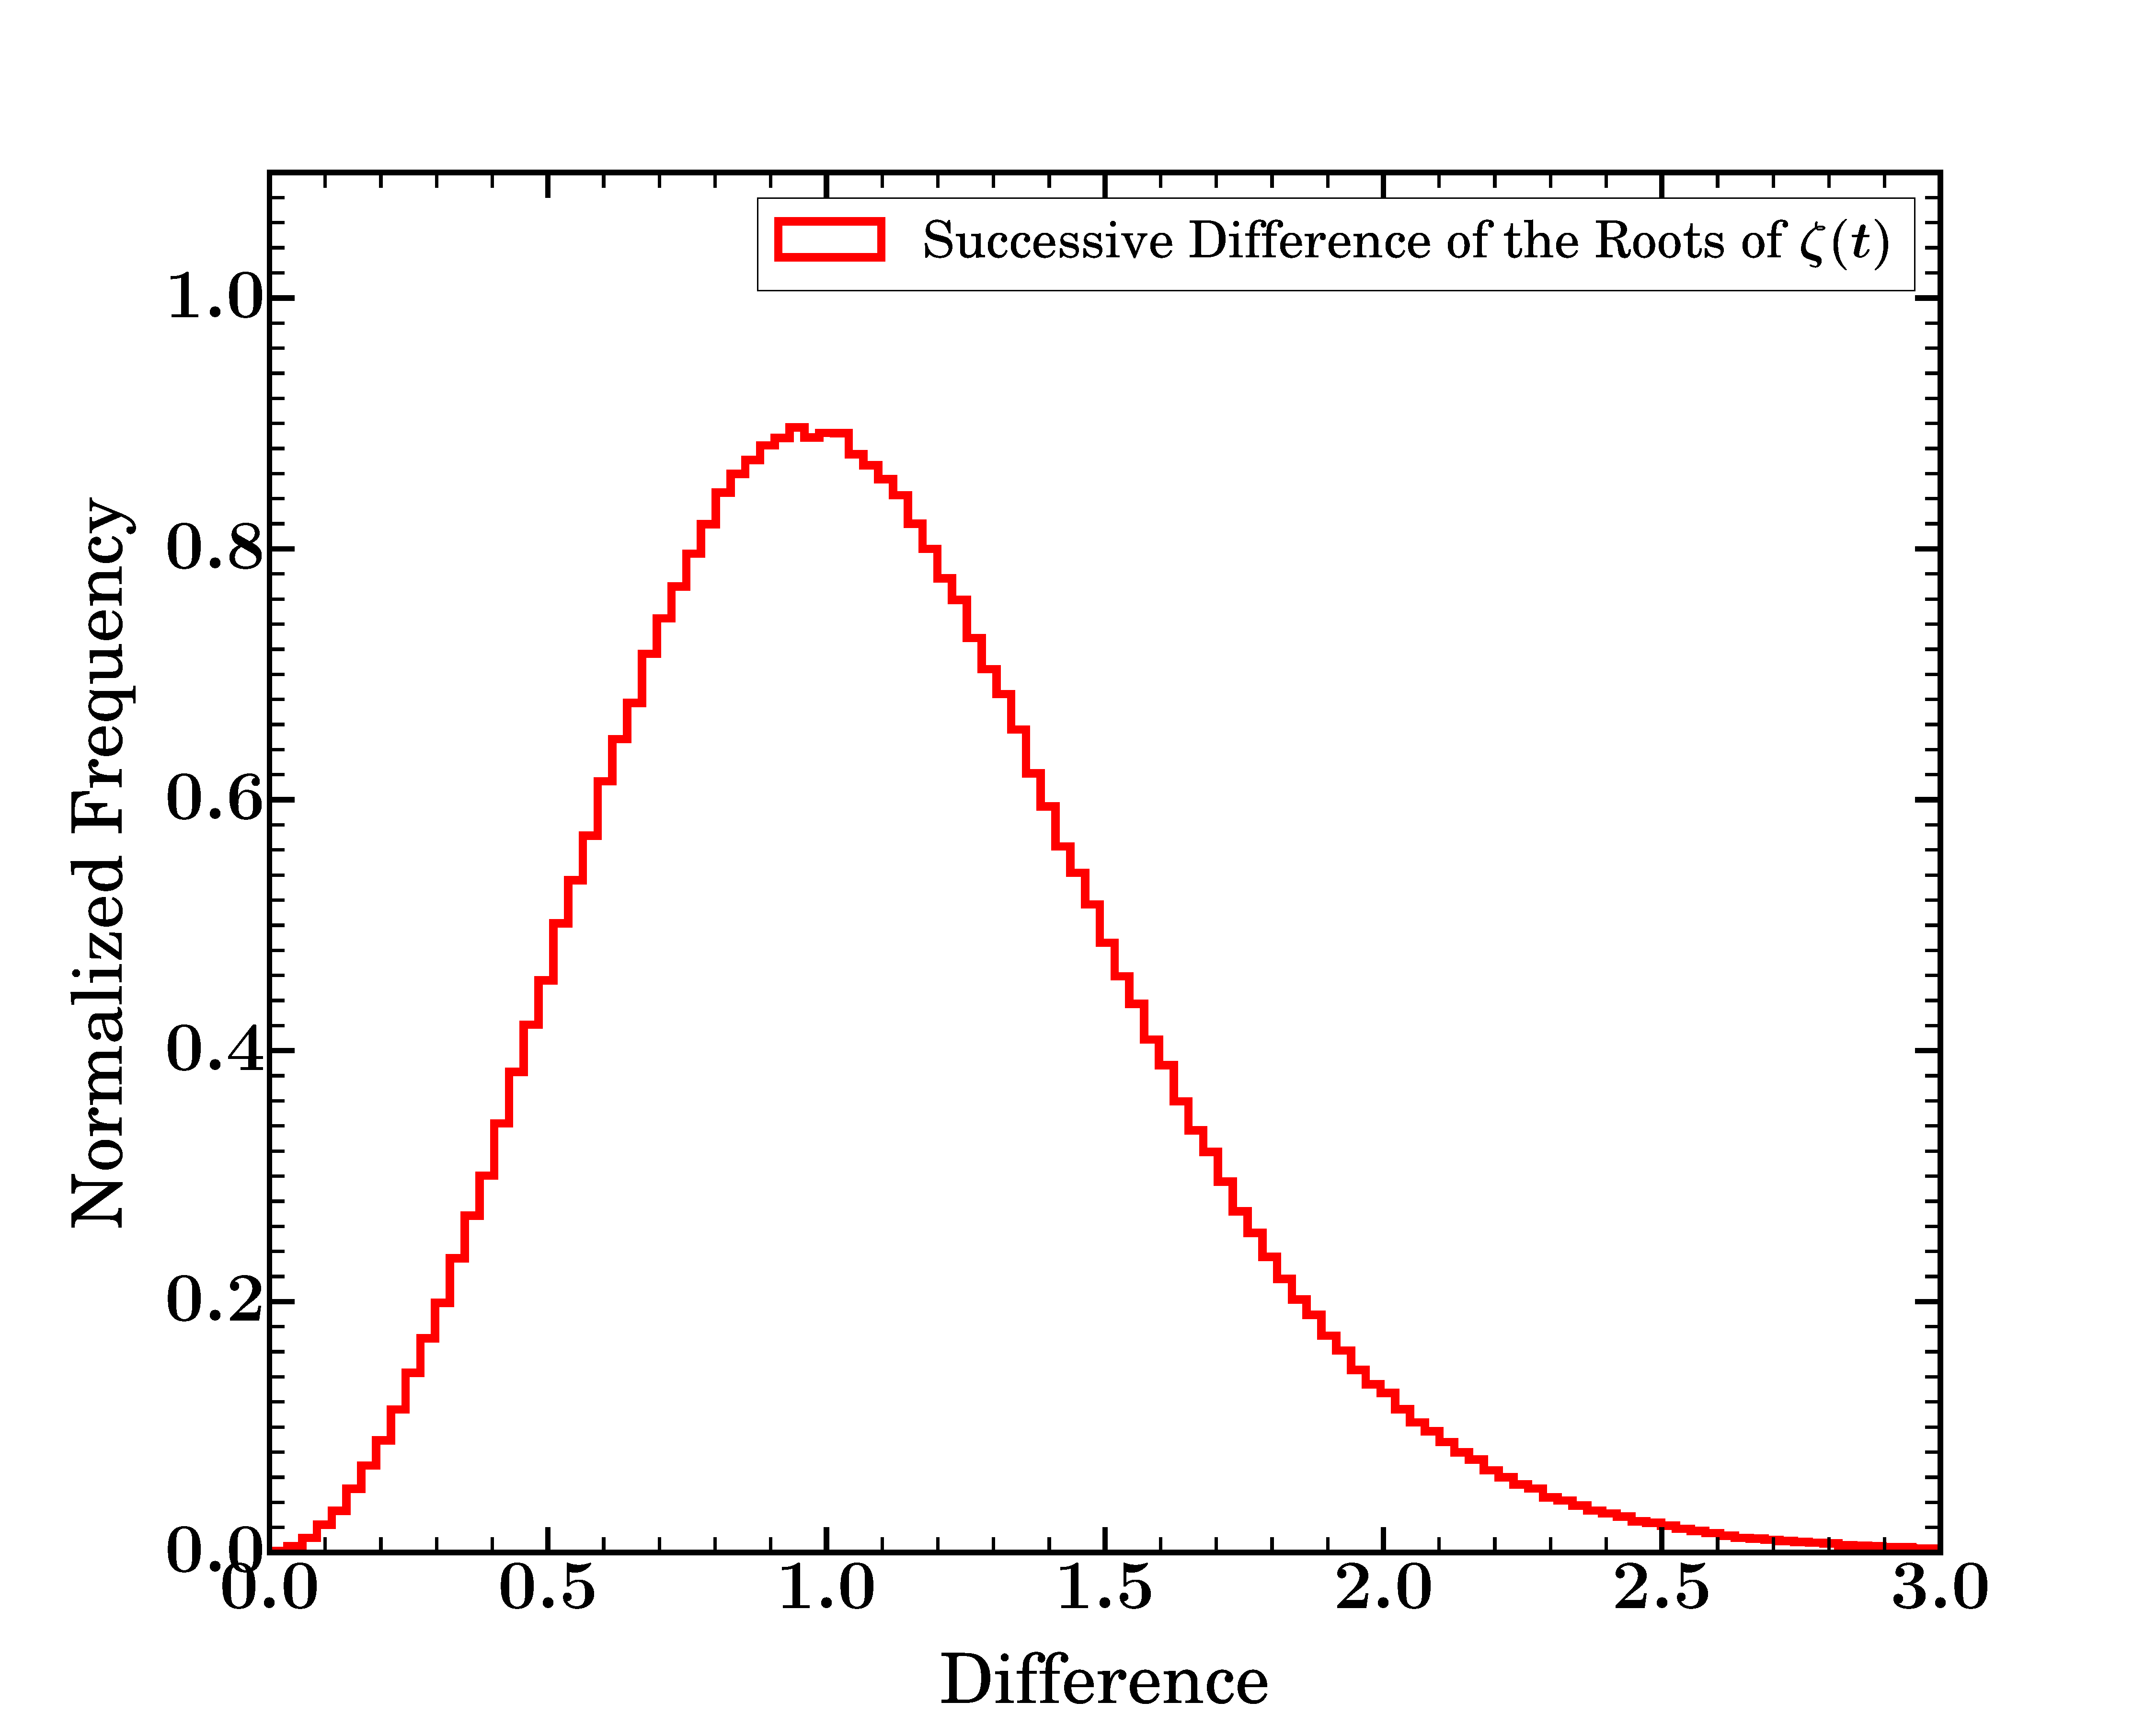
\includegraphics[width=\columnwidth]{figures/zeta_zeros_normalized_differences.pdf}
\caption{Distribution of successive differences of the first 2 million non-trivial zeros of $\zeta(t)$. The differences have been normalized so that the mean is 1.}
\label{fig:zeta_zeros_normalized_differences}
\end{figure}



\section{Random Matrices}
A random matrix is a matrix whose elements are random variables. Two most commonly studied types of random matrices are Gaussian Orthogonal Ensemble (GOE) and Gaussian Unitary Ensemble (GUE). 

\subsection{Gaussian Orthogonal Enseblme (GOE)}
A Gaussian Orthogonal Ensemble is a set of $n \times n$ real-valued symmetric matrices $H_n$ whose Gaussian measure has the density, 
$$
\frac{1}{Z_{\mathrm{GOE}}} e^{ - \frac{n}{4} \mathrm{tr}(H^2) } \;.
$$
GOEs model Hamiltonians with time-reversal symmetry. 

Consider the ordered sequence of eigenvalues of $H_n$, $\lambda_1 < \lambda_2 < \ldots \lambda_{n - 1} < \lambda_n$. Define $s = \frac{\lambda_{i + 1} - \lambda_{i}}{ \left< s \right> }$. Then, the probability distribution on $s$ is given by, 
$$
p_{\mathrm{GOE}}(s) = \frac{\pi}{2} s e^{- \frac{\pi}{4} s^2 }
$$

\begin{figure}
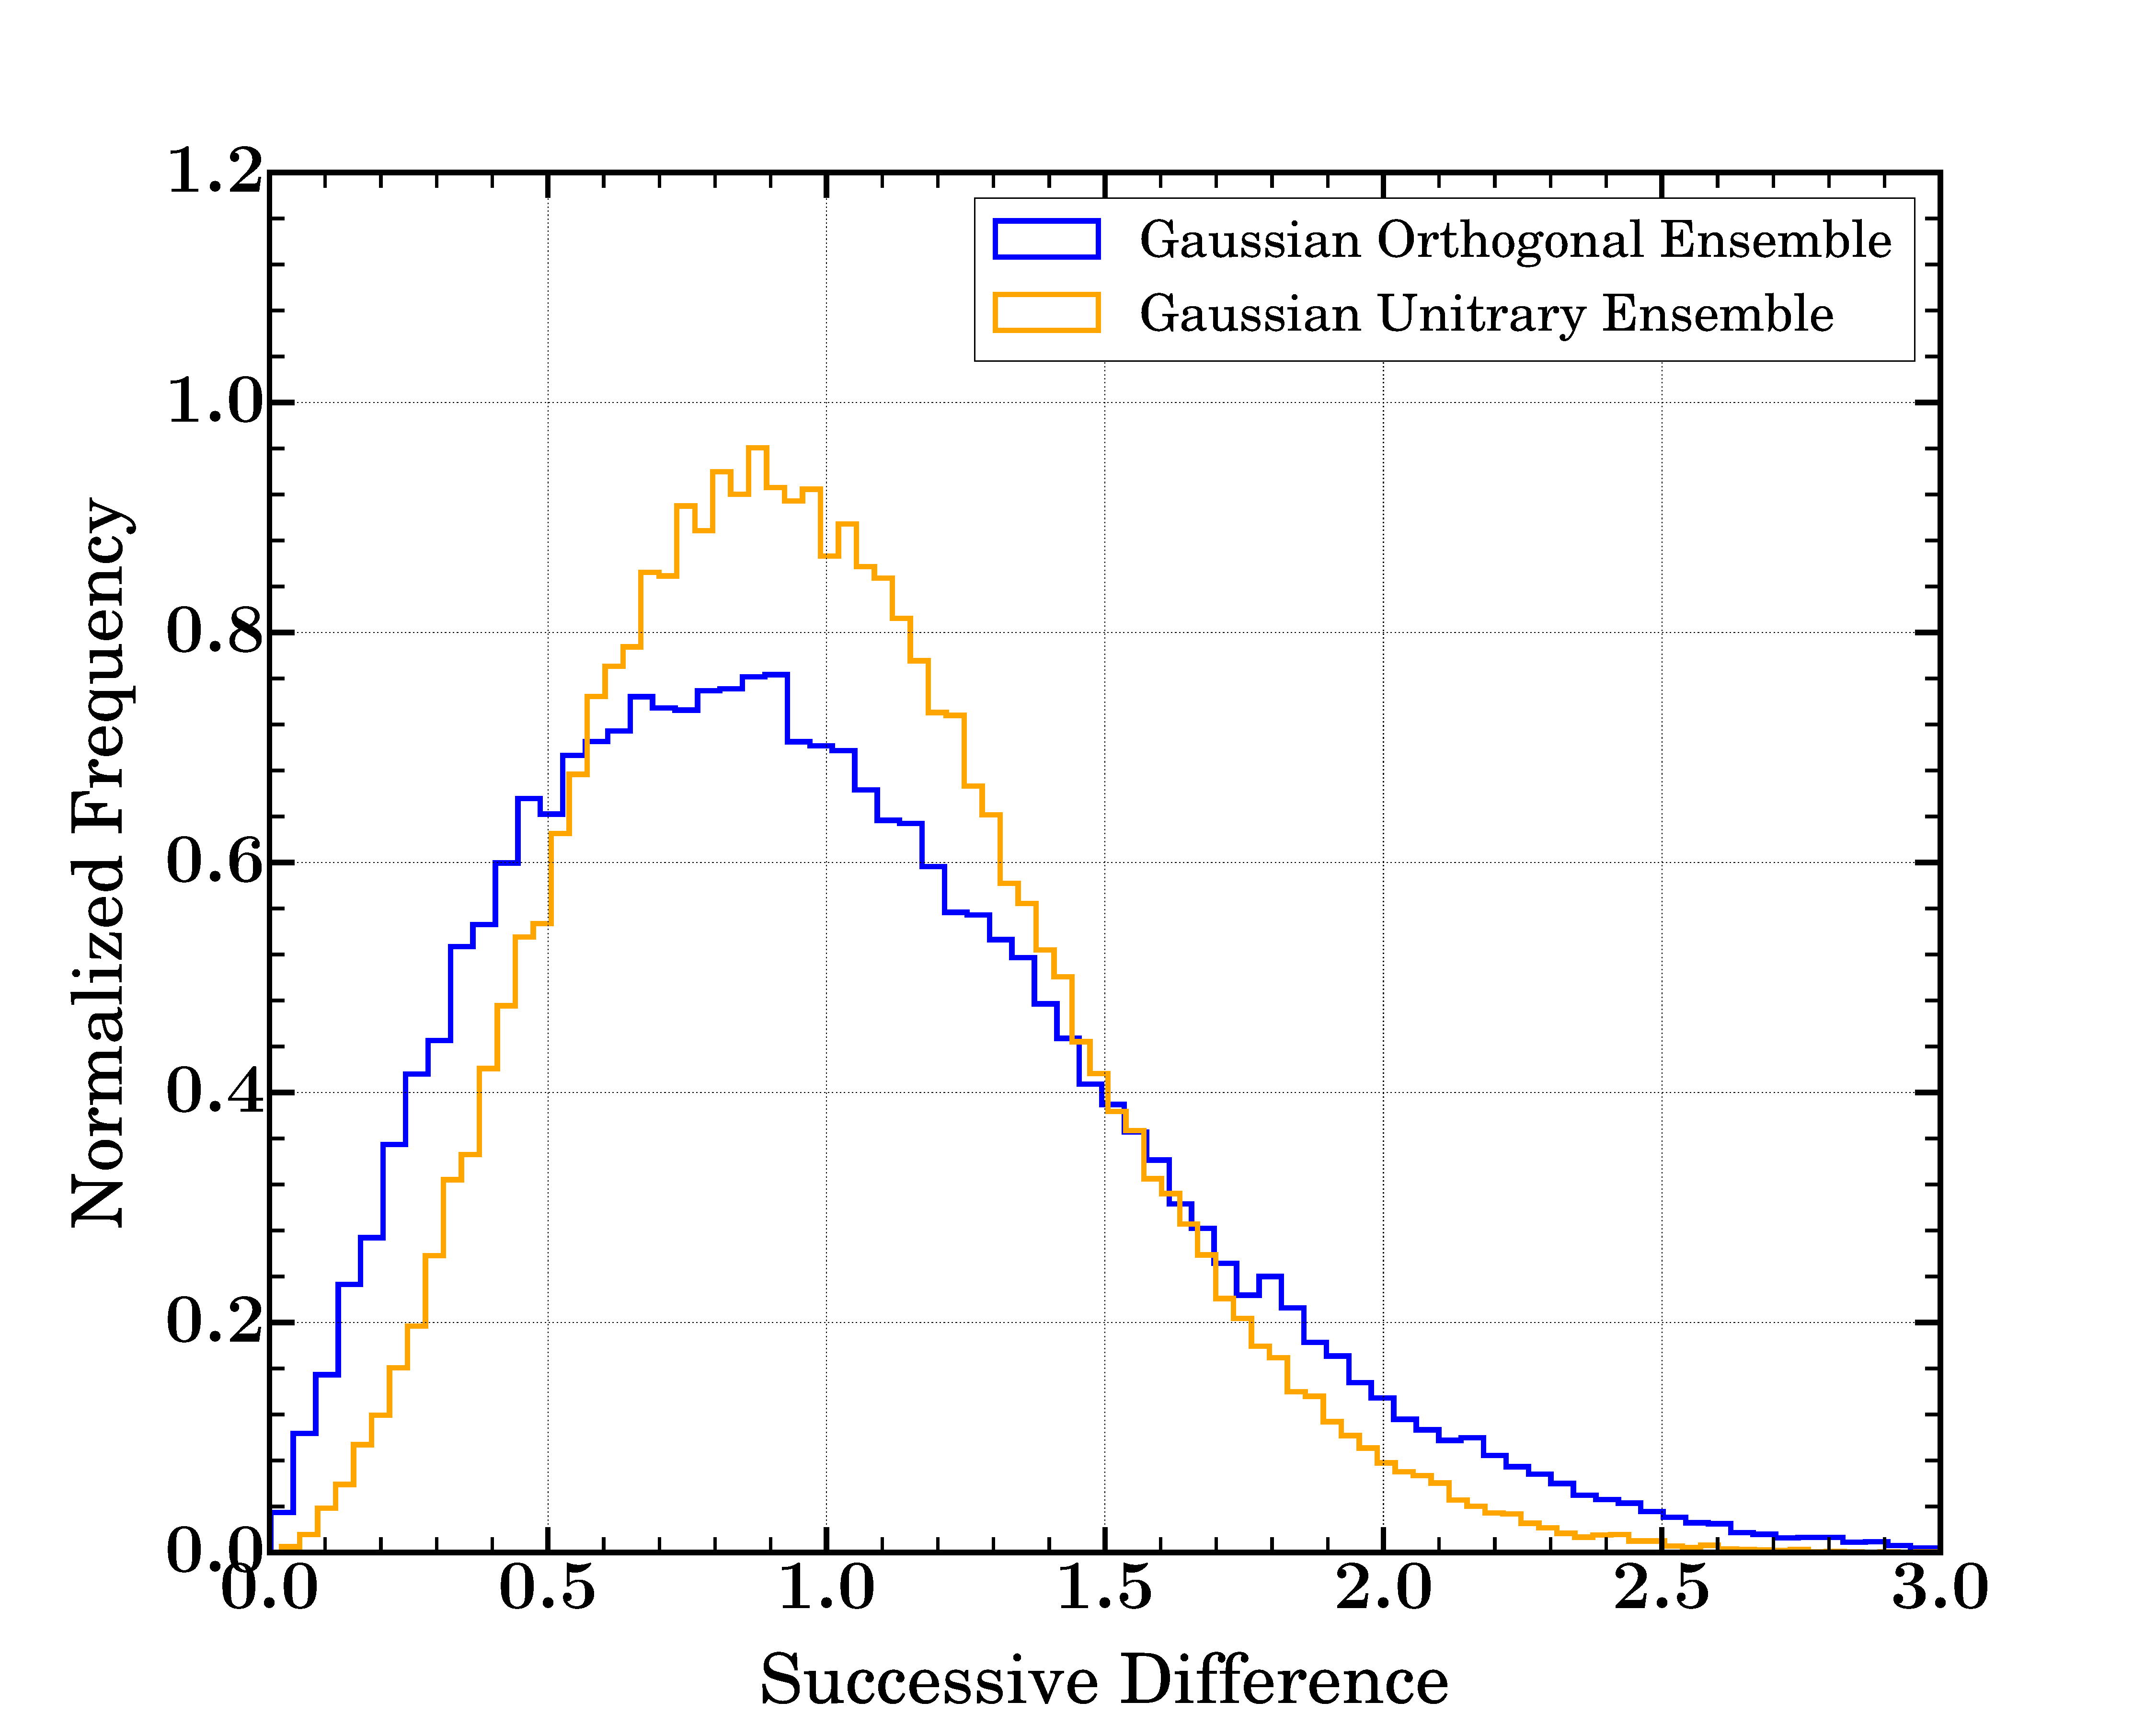
\includegraphics[width=\columnwidth]{figures/random_matrices_eigenvalues_differences.pdf}
\caption{Succesive eigenvalue differences for Gaussian Orthogonal and Gaussian Unitary Ensembles of $100\;\mathrm{K}$ $25 \times 25$ matrices. Each difference corresponds to $\lambda_{\lceil N \rceil + 1} - \lambda_{ \lceil N \rceil}$.}
\label{fig:random_matrices_eigenvalues_differences}
\end{figure}

\subsection{Gaussian Unitary Enseblme (GUE)}
A Gaussian Unitary Ensemble is a set of $n \times n$ Hermitian matrices $H_n$ whose Gaussian measure has the density, 
$$
\frac{1}{Z_{\mathrm{GUE}}} e^{ - \frac{n}{2} \mathrm{tr}(H^2) } \;,
$$
with $Z_{\mathrm{GUE}} = 2^{ \pi / 2} \pi^{n^2 / 2}$. GUEs model Hamiltonians lacking time-reversal symmetry. 

For GUEs, the probability distribution on $s$, is given by, 
$$
p_{\mathrm{GUE}}(s) = \frac{32}{\pi^2} s^2 e^{- \frac{4}{\pi} s^2 }
$$

\section{Riemann Hypothesis}
The Riemann hypothesis conjectures that all non-trivial roots of the zeta function have real-part $1/2$. It was proposed by Riemann in 1859 in the same paper where he introduced the zeta funciton, ``On the Number of Primes Less Than a Given Magnitude''.

The Riemann hypothesis is arguably one of the most important unsolved problems in mathematics. Several approaches to proving it has been attempted but none has succedded so far. Numerically, it has been tested to be true for the first $10^{13}$ roots by X. Gourdon and Patrick Demichel \cite{}. However, numerical verification, no matter to how large values of $t$, can not be considered to be a compelling argument for a mathematical hypothesis to be true. One notable example is related to Skewes' number where a related conjecture breaks down for the first time at a number around $10^{316}$. 

\section{Hilbert-Polya Conjecture}
The Hilbert-Polya conjecture suggests that the Riemann hypothesis would be true if the imaginary parts of the zeros of the zeta function correspond to the eigenvalues of some unbounded Hermitian operator. This came out of a letter to Andrew Odlyzko, in 1982, in which Polya wrote that he was asked by Edmund Landau for a physical reason why the Riemann hypothesis must be true, to which he proposed the conjecture. 

The eigenvalues of a physical quantum operator are all real values and Hermitian operators are guaranteed to have real eigenvalues. This means, a physical way of proving the Riemann hypothesis would be to try to find a quantum mechanical operator whose eigenvalues (which will be all real) coincide with the imaginary parts of the non-trivial zeros of the Riemann zeta function. Finding any such quantum mechanical operator would be a proof of the Hilber-Polya conjecture and the Riemann hypothesis both. So in a sense, the Hilbert-Polya conjecture is just an alternate formulation of the Riemann hypothesis that makes it possible to try to find a physical proof of the Riemann hypothesis. 


It's important to note that there are infinitely many non-trivial zeros the $\zeta(t)$ \ref{} and so, if such a Hermitian matrix does exist, as conjectured by the Hilbert-Polya conjecture, that matrix would have to be infinite-dimensional. Of course, that's not a problem since most quantum mechanical operators, even the simplest ones like say the Hamiltonian corresponding the a simple harmonic oscillator, have matrix forms where the dimension is infinite-dimensional. But it's something that one needs to be aware of since, for example, because no numerical calculations can go until infinity, numerical methods of finding / testing such quantum systems must be careful, and certain properties, the most notable example being the commutation relationship, won't be valid when we arrest the matrix representation to a finite size for numerical computations. The first one of this will be particularly important in Section. \ref{} where we discuss one such possible quantum system. 

Very broadly speaking, there are now two approaches to prove the Riemann hypothesis. Through the Hilber-Polya conjecture, we've reduced the problem to finding some quantum mechanical system with a specific property. Because the operator (most likely the Hamiltonian) needs to be Hermitian, it's reasonable to expect, though this certainly does not have to be true, would be some function of the most common physical quantum mechanical operators. Finiding such an operator and testing whether or not its eigenvalues corresponds to the imaginary part of the non-trivial zeros of $\zeta(t)$ could be done numerically or we could try to find an analytical expression for those eigenvalues of our operator, in which case the analytical form would probably reduce to essentially one of the already known forms for $\zeta(t)$ equated to 0. Of course, it's not unconceivable that this would lead to an alternate expression for $\zeta(t)$ but nevertheless, the Hilbert-Polya conjecture opens up the door for attempts to prove the Riemann hypothesis in an alternate way. 


\section{$\zeta(t)$ and Random Matrices}
If we're to prove the Riemann hypothesis, a careful study of the distribution of the non-trivial zeros of $\zeta(t)$ is crucial. In 1973, Montgomery conjectured that there mught be some possible connection between those non-trivial zeros and random matrices. Of particular interest is to study the distribution of successive differences of eigenvalues of the Gaussian Unitary Ensemble (GUE) and compare it to the successive differences of the non-trivial zeros of the zeta function. 

It's interesting to note that the Gaussian Unitary Ensemble is a realization of every possible Hermitian matrices (assuming the ensemble size goes to infinity). But, through the Hilbert-Polya conjecture, there seems to be at least some connection between the eigenvalues of some such Hermitian matrix and the non-trivial zeros of the zeta function. 

We need to choose some variable that is well-defined for both the GUEs and the distribution of the zeros of $\zeta(t)$ and then we can compare that variable for the two cases. One such possible variable is to consider the 2-point correlation function $R_2(E_1, E_2)$ which gives the probability density function of finding an eigenvalue of $H$ at each of the values $E_1, E_2$.  Montogomery, in 1972, showed that the 2-point correlation function for GUEs is given by,
$$
R_2(r) = 1 - \left[ \frac{ \sin{\pi r} }{\pi r} \right]^2 \;,
$$
and the 2-point correlation function for the Riemann zeros is, 
$$
R_{\zeta, 2}(r) = 1 - \left[ \frac{ \sin{\pi r} }{\pi r} \right]^2 \;.
$$
This is remarkable since this implies that \at{What does this imply?}

Another interesting variable to comapre is the level-spacing of the zeros and the eigenvalues. What this means is, we could compute the successive differences (after sorting the eigenvalues / zeros) and compare them, subject to appropriate normalization. This is exactly the probability distribution we defined in \ref{} as $p_{\mathrm{ensemble}}(s)$. We normalize both the distributions so that the mean is 1, as that makes it easy to compare them. 

\begin{figure}
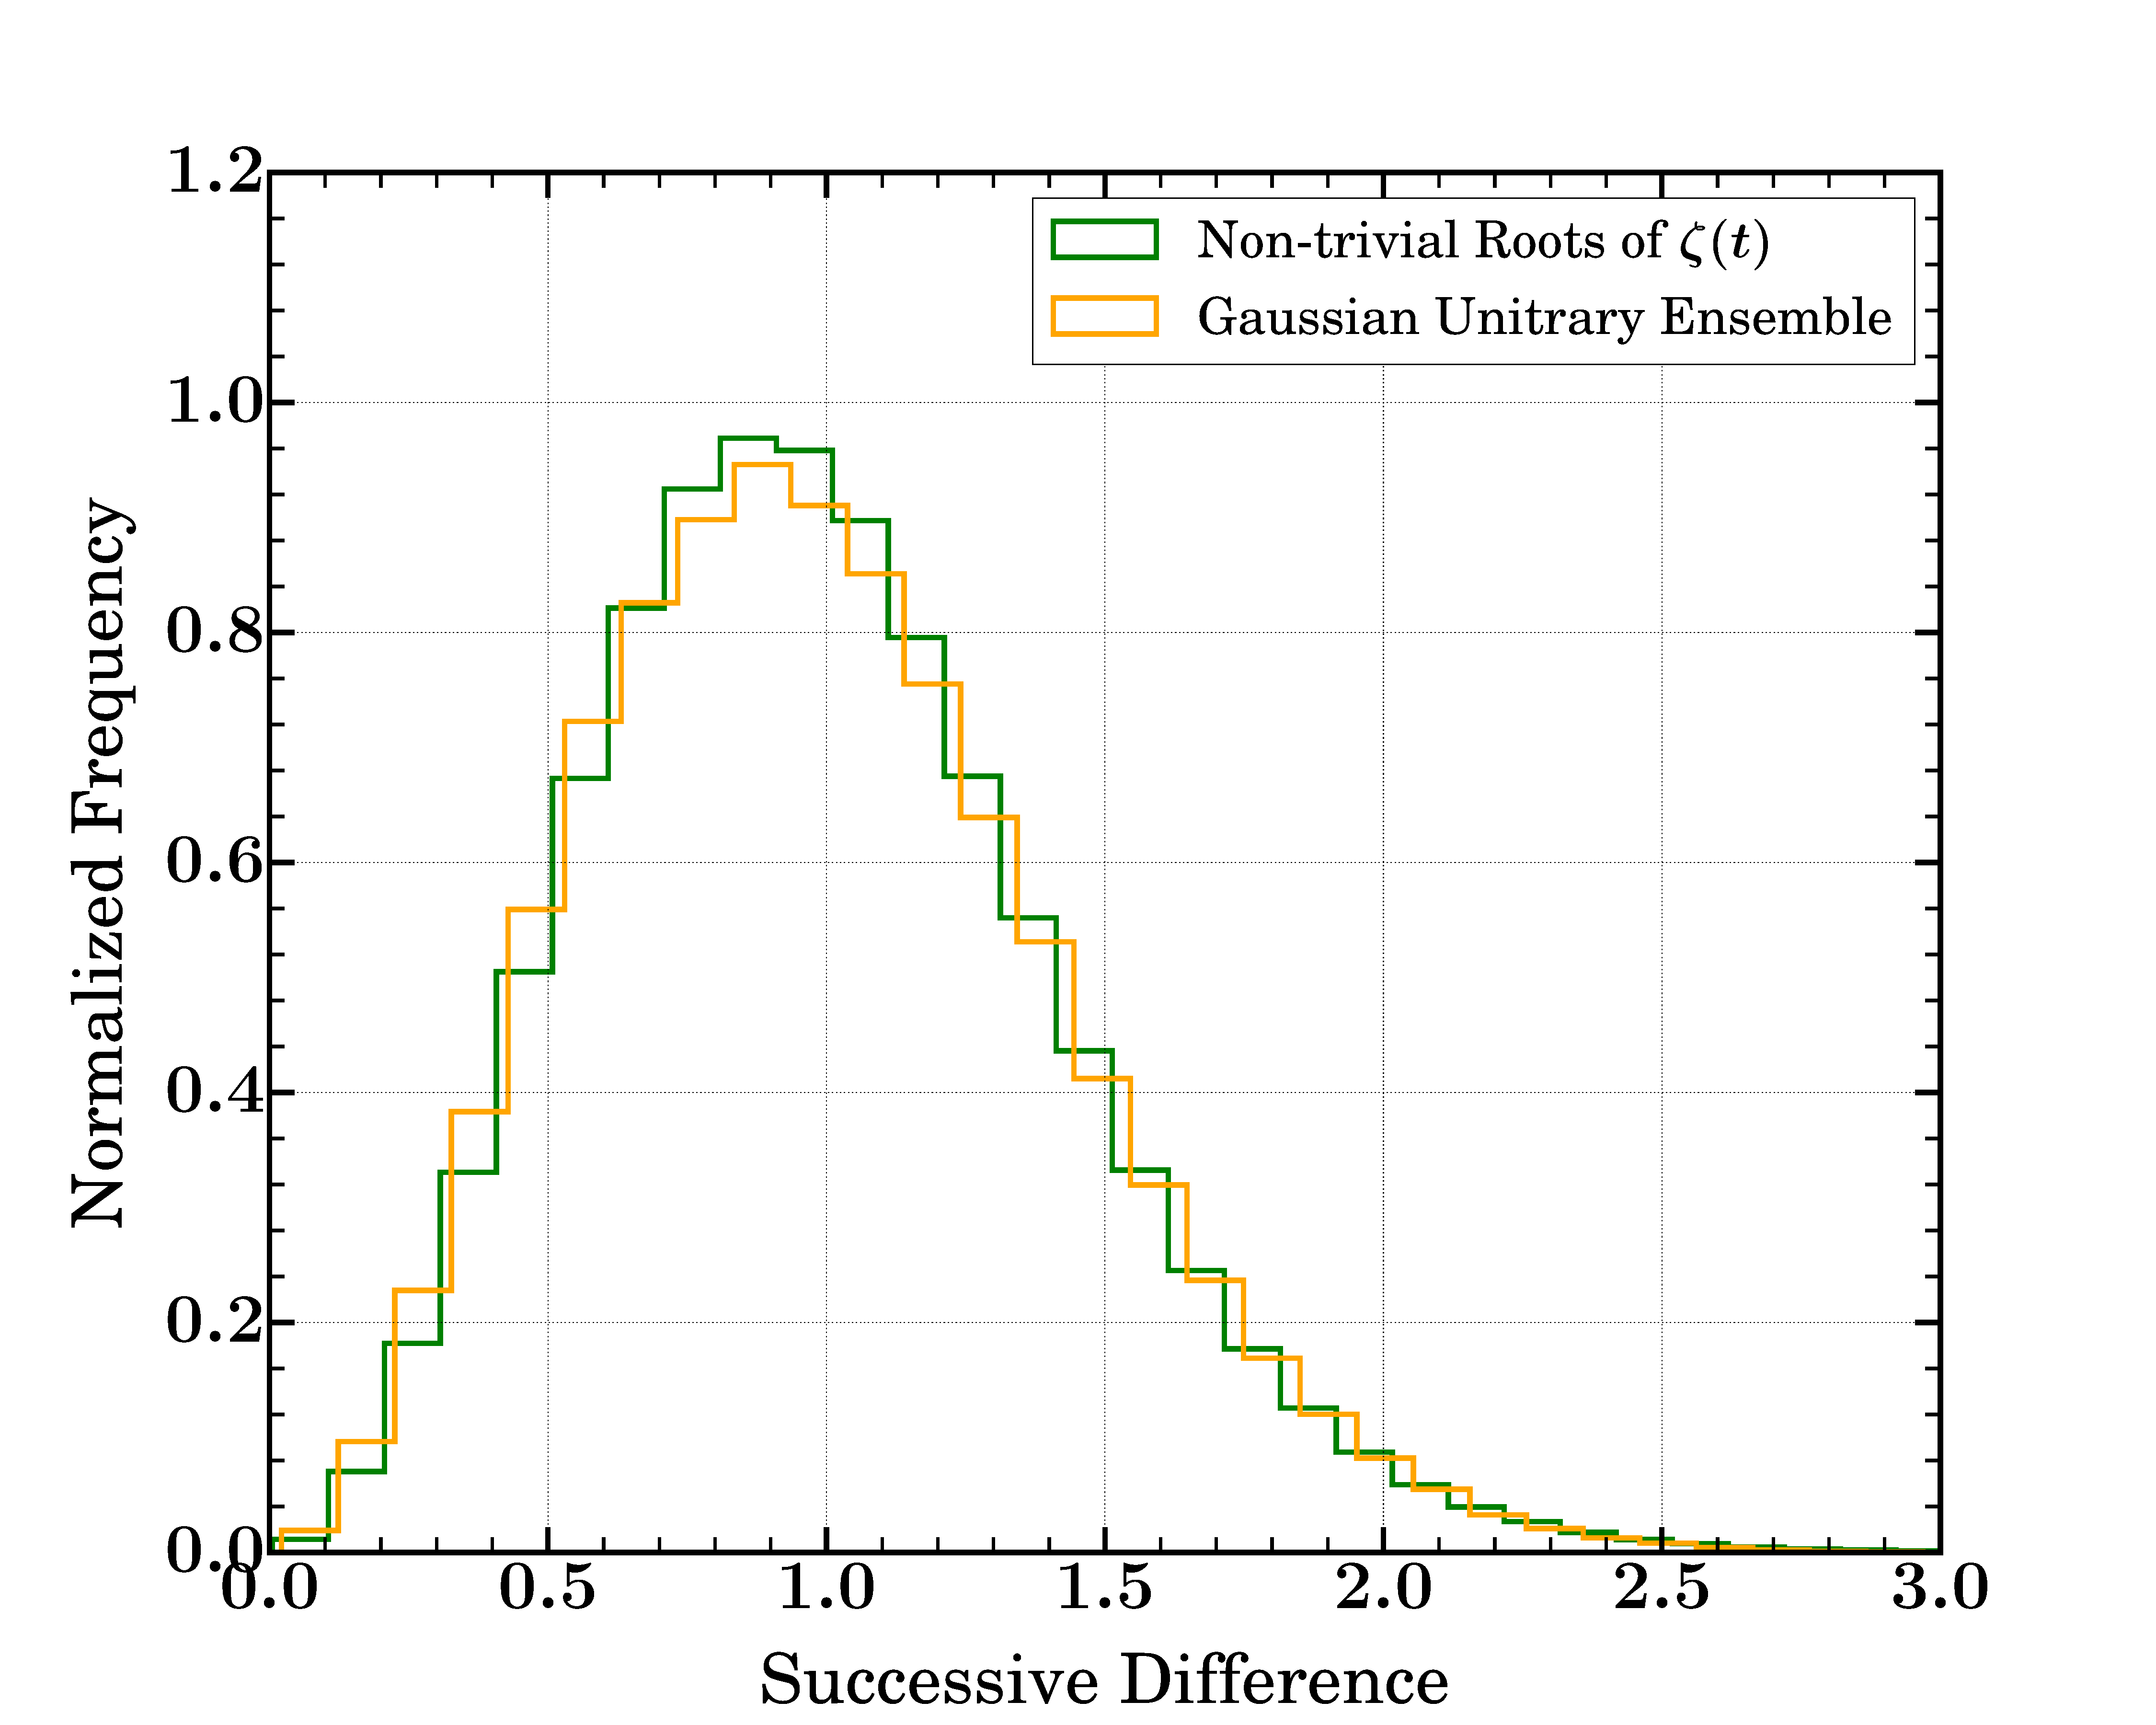
\includegraphics[width=\columnwidth]{figures/GUE_eigenvalues_and_zeros_differences.pdf}
\caption{Succesive eigenvalue differences for Gaussian Unitary Ensembles of $100\mathrm{K}$ $25 \times 25$ matrices and the first 2M non-trivial zeros of $\zeta(t)$. For GUE, each difference corresponds to $\lambda_{\lceil N \rceil + 1} - \lambda_{ \lceil N \rceil}$. Both distributions have been normalized so that their mean is 1. }
\label{fig:random_matrices_eigenvalues_differences}
\end{figure}

\section{Quantum Mechanics}
Michael Berry and Jonathan Keating have conjectured that the Hilbert-Polya Hamiltonian $H$ is some quantization of the Hamiltonian $xp$. We'll consider one such possible quantization and discuss it at length in this secion. Let's define:
\be
H = \frac{1}{2} \left( x p + p x \right) = -i \left( x\frac{ \partial}{\partial x} + \frac{1}{2} \right)
\ee
For a simple harmonic oscialltor, $x$ and $p$ can be written in terms of raising and lowering operators $a$ and $a^{\dagger}$ as,
\be
x = \sqrt{\frac{ \hbar }{ 2 m \omega }} (a + a^{\dagger} )\,;
p = i \sqrt{ \frac{m \omega \hbar }{ 2 } } ( a^{\dagger} - a )
\ee
Let's ignore the factors in the front and just consider the linear combination of $a$ and $a^{\dagger}$ along with the imaginary unit. Using this expansion, it's fairly straightfoward to see that,
\be
H = \frac{1}{2} \left( xp + px \right) = i \left[ ( a^{\dagger} )^2 - (a)^2 \right]
\ee

$a^{\dagger}$ and $a$ has infinite-dimensional matrix representations as follows:

\[
a^{\dagger}
=
\begin{bmatrix}
    0        & 0        & 0        &  0       & \dots  \\
    \sqrt{1} & 0        & 0        &  0       & \dots   \\
    0        & \sqrt{2} & 0        &  0       &\dots   \\
    0        & 0        & \sqrt{3} &  0       & \dots   \\
    0        & 0        & 0        & \sqrt{4} & \dots   \\
    \vdots & \vdots & \vdots & \ddots & \vdots \\
    \hdots & \hdots & \hdots & \hdots & \hdots \\
\end{bmatrix} \, ,
a
=
\begin{bmatrix}
    0        & \sqrt{1} & 0        &  0       & \dots  \\
    0        & 0        & \sqrt{2} &  0       & \dots   \\
    0        & 0        & 0        & \sqrt{3} &\dots   \\
    0        & 0        & 0        &  0       & \dots   \\
    0        & 0        & 0        &  0 & \dots   \\
    \vdots & \vdots & \vdots & \ddots & \vdots \\
    \hdots & \hdots & \hdots & \hdots & \hdots \\
\end{bmatrix}
\]
For our computation, we will consider $N$ dimensional matrices instead of infinite dimensional. 

Let's study what the eigevalues of $H$ look like. Because $a$ and $a^{\dagger}$ are sparse matrices, computing their eigenvalues, even for large $N$, is not too bad. 

We again have to make a choice of what properties of the operator $H$ (and its eigenvalues) we want to study. The obvious choice is to study the successive difference of eigenvalues like we did for random matrices and the non-trivial zeros of $\zeta(t)$. Figure \ref{fig:everything} shows a plot. It's interesting to note that \at{what?}


\begin{figure}
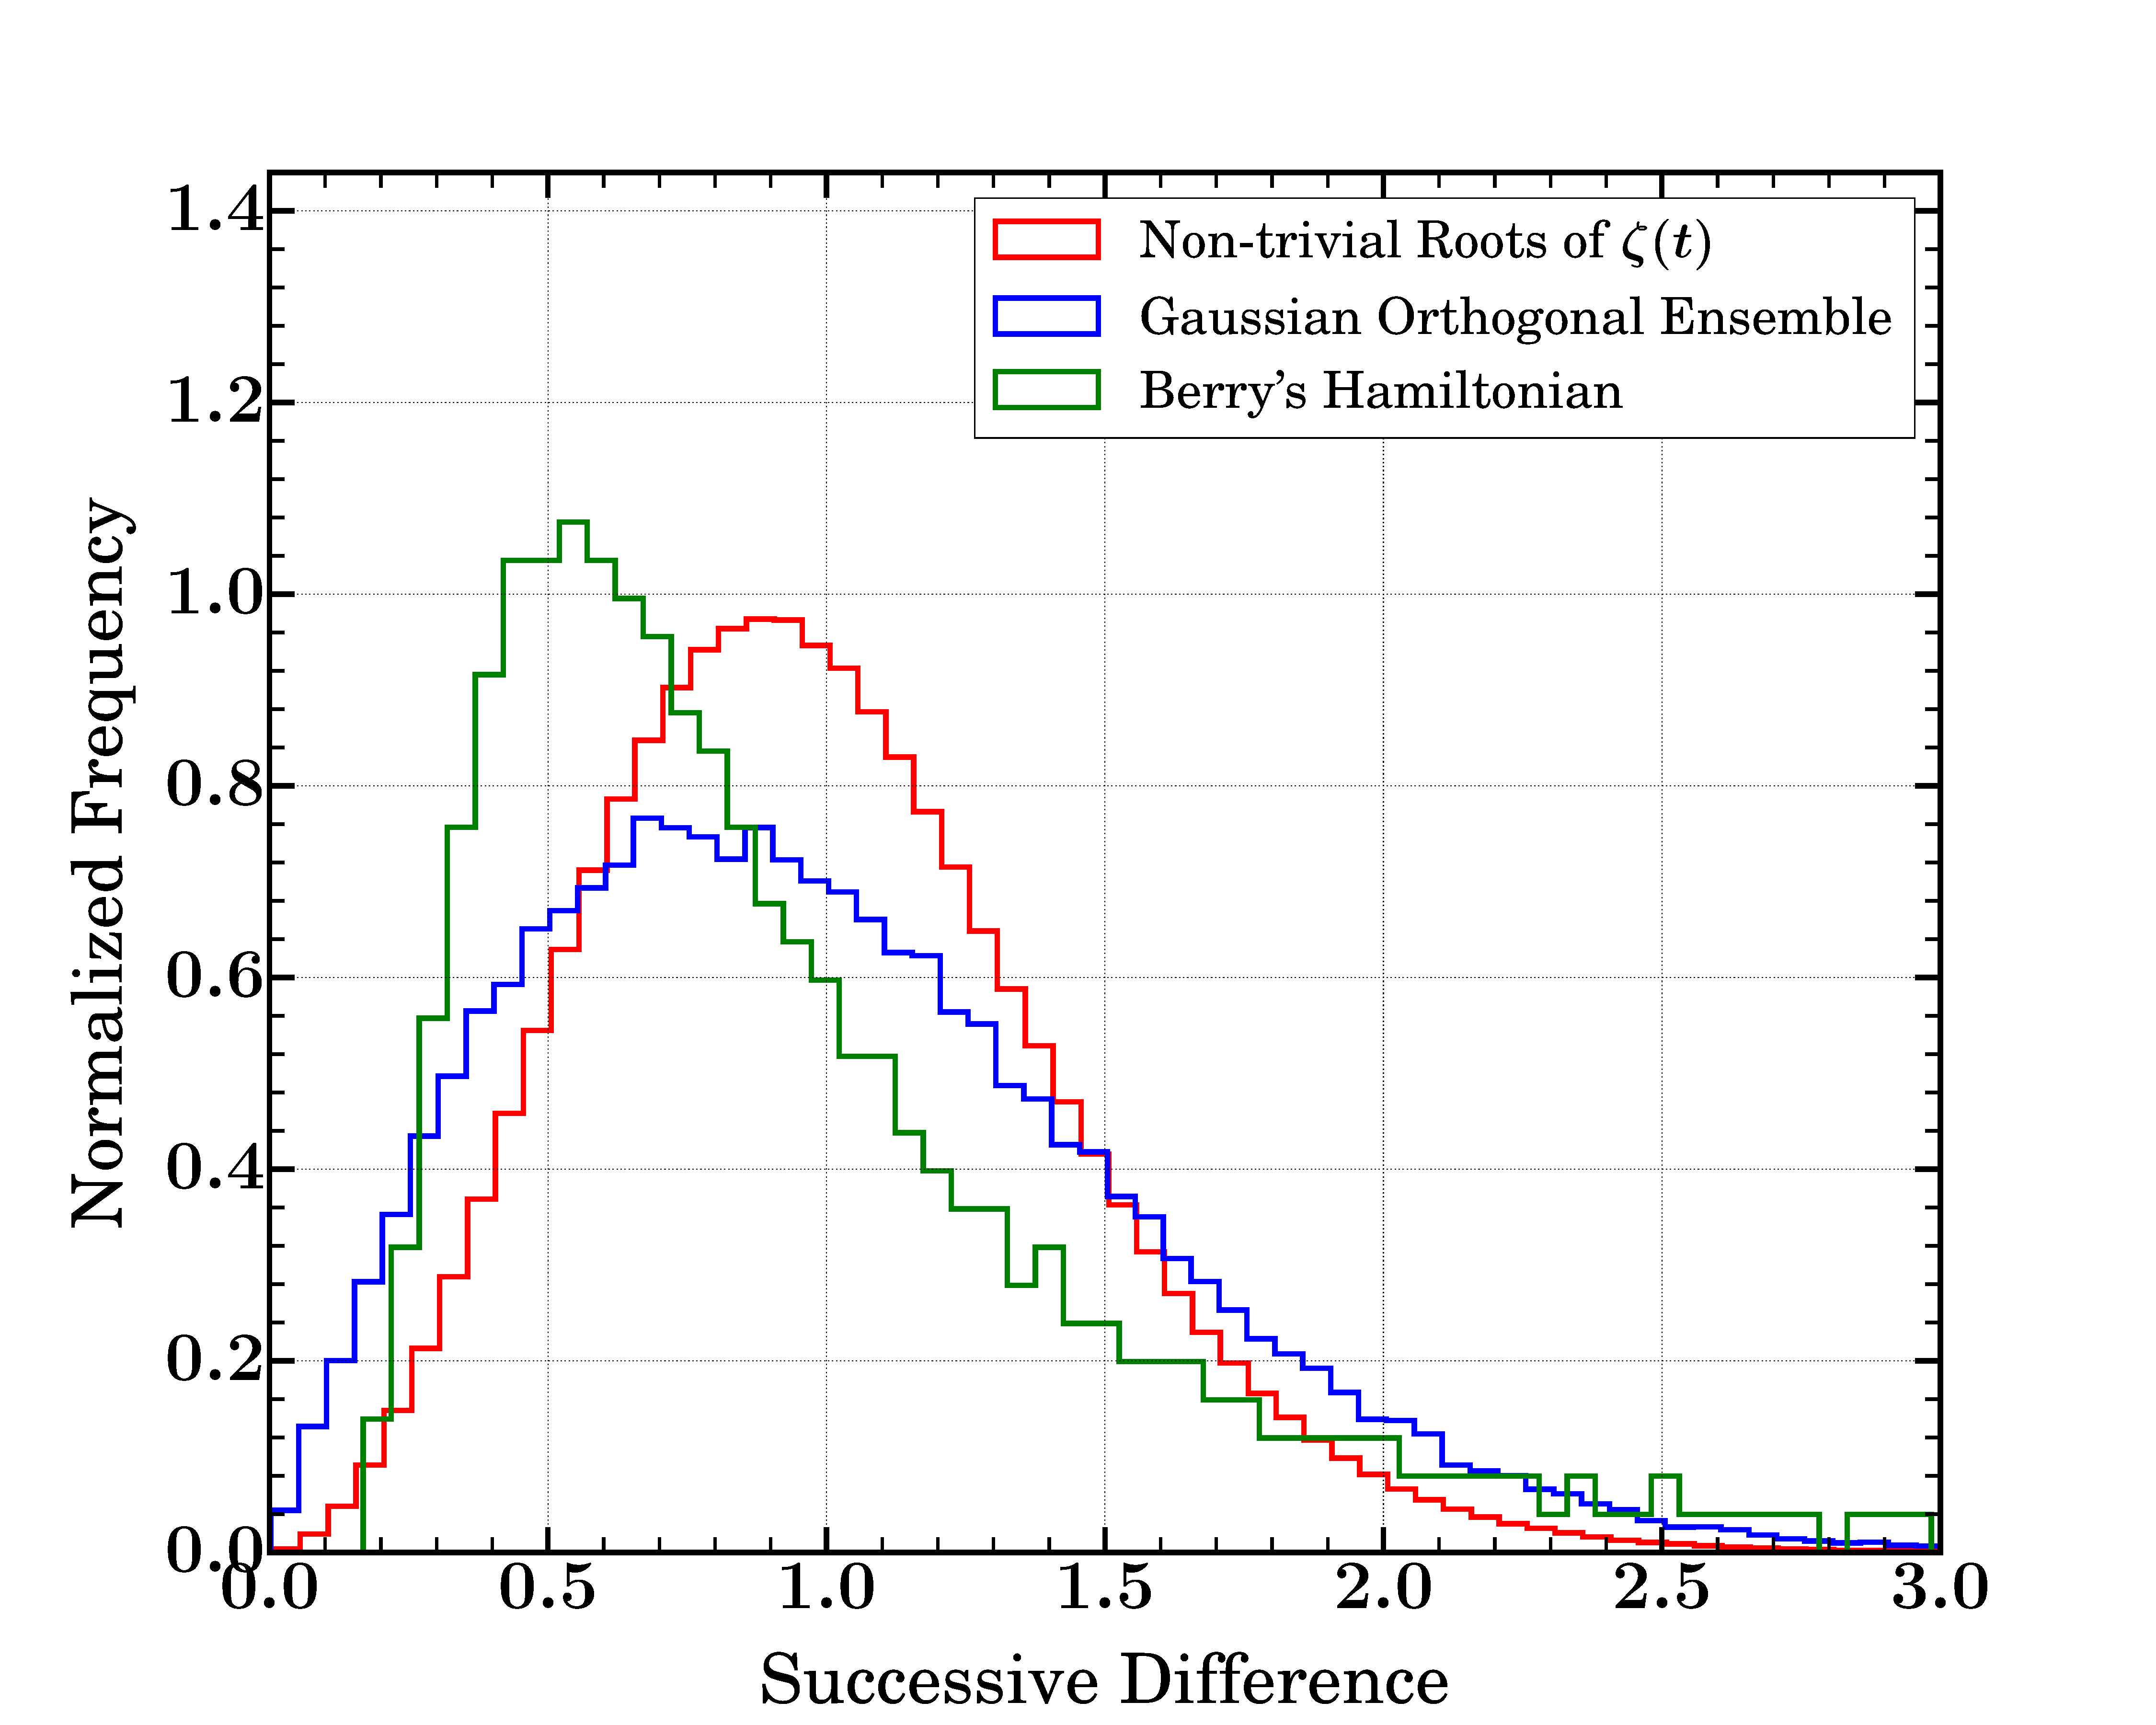
\includegraphics[width=\columnwidth]{figures/everything.pdf}
\caption{Succesive eigenvalue differences for Gaussian Orthogonal Ensembles of $100\mathrm{K}$ $25 \times 25$ matrices, the first 2M non-trivial zeros of $\zeta(t)$ and the Berry Hamiltonian, $H$. For $H$, we consider a $1000 \times 1000$ matrix representation. For GOE, each difference corresponds to $\lambda_{\lceil N \rceil + 1} - \lambda_{ \lceil N \rceil}$. All distributions have been normalized so that their mean is 1. }
\label{fig:everything}
\end{figure}

An interesting feature of the plot in Figure. \ref{fig:everything} is that, while the distributions for the non-trivial roots and GUE seems to go down all the way to 0, there seems to be a finite cut for the eigenvalue difference for Berry's Hamiltonian $H$. The existence of this finite cut isn't a remarkable property by itself since this just means that there is no degeneracy for the Hamiltonian we're considering. What's interesting though is that, this cut seems to depend on the size of the matrix representation we choose $N$.

\begin{figure}
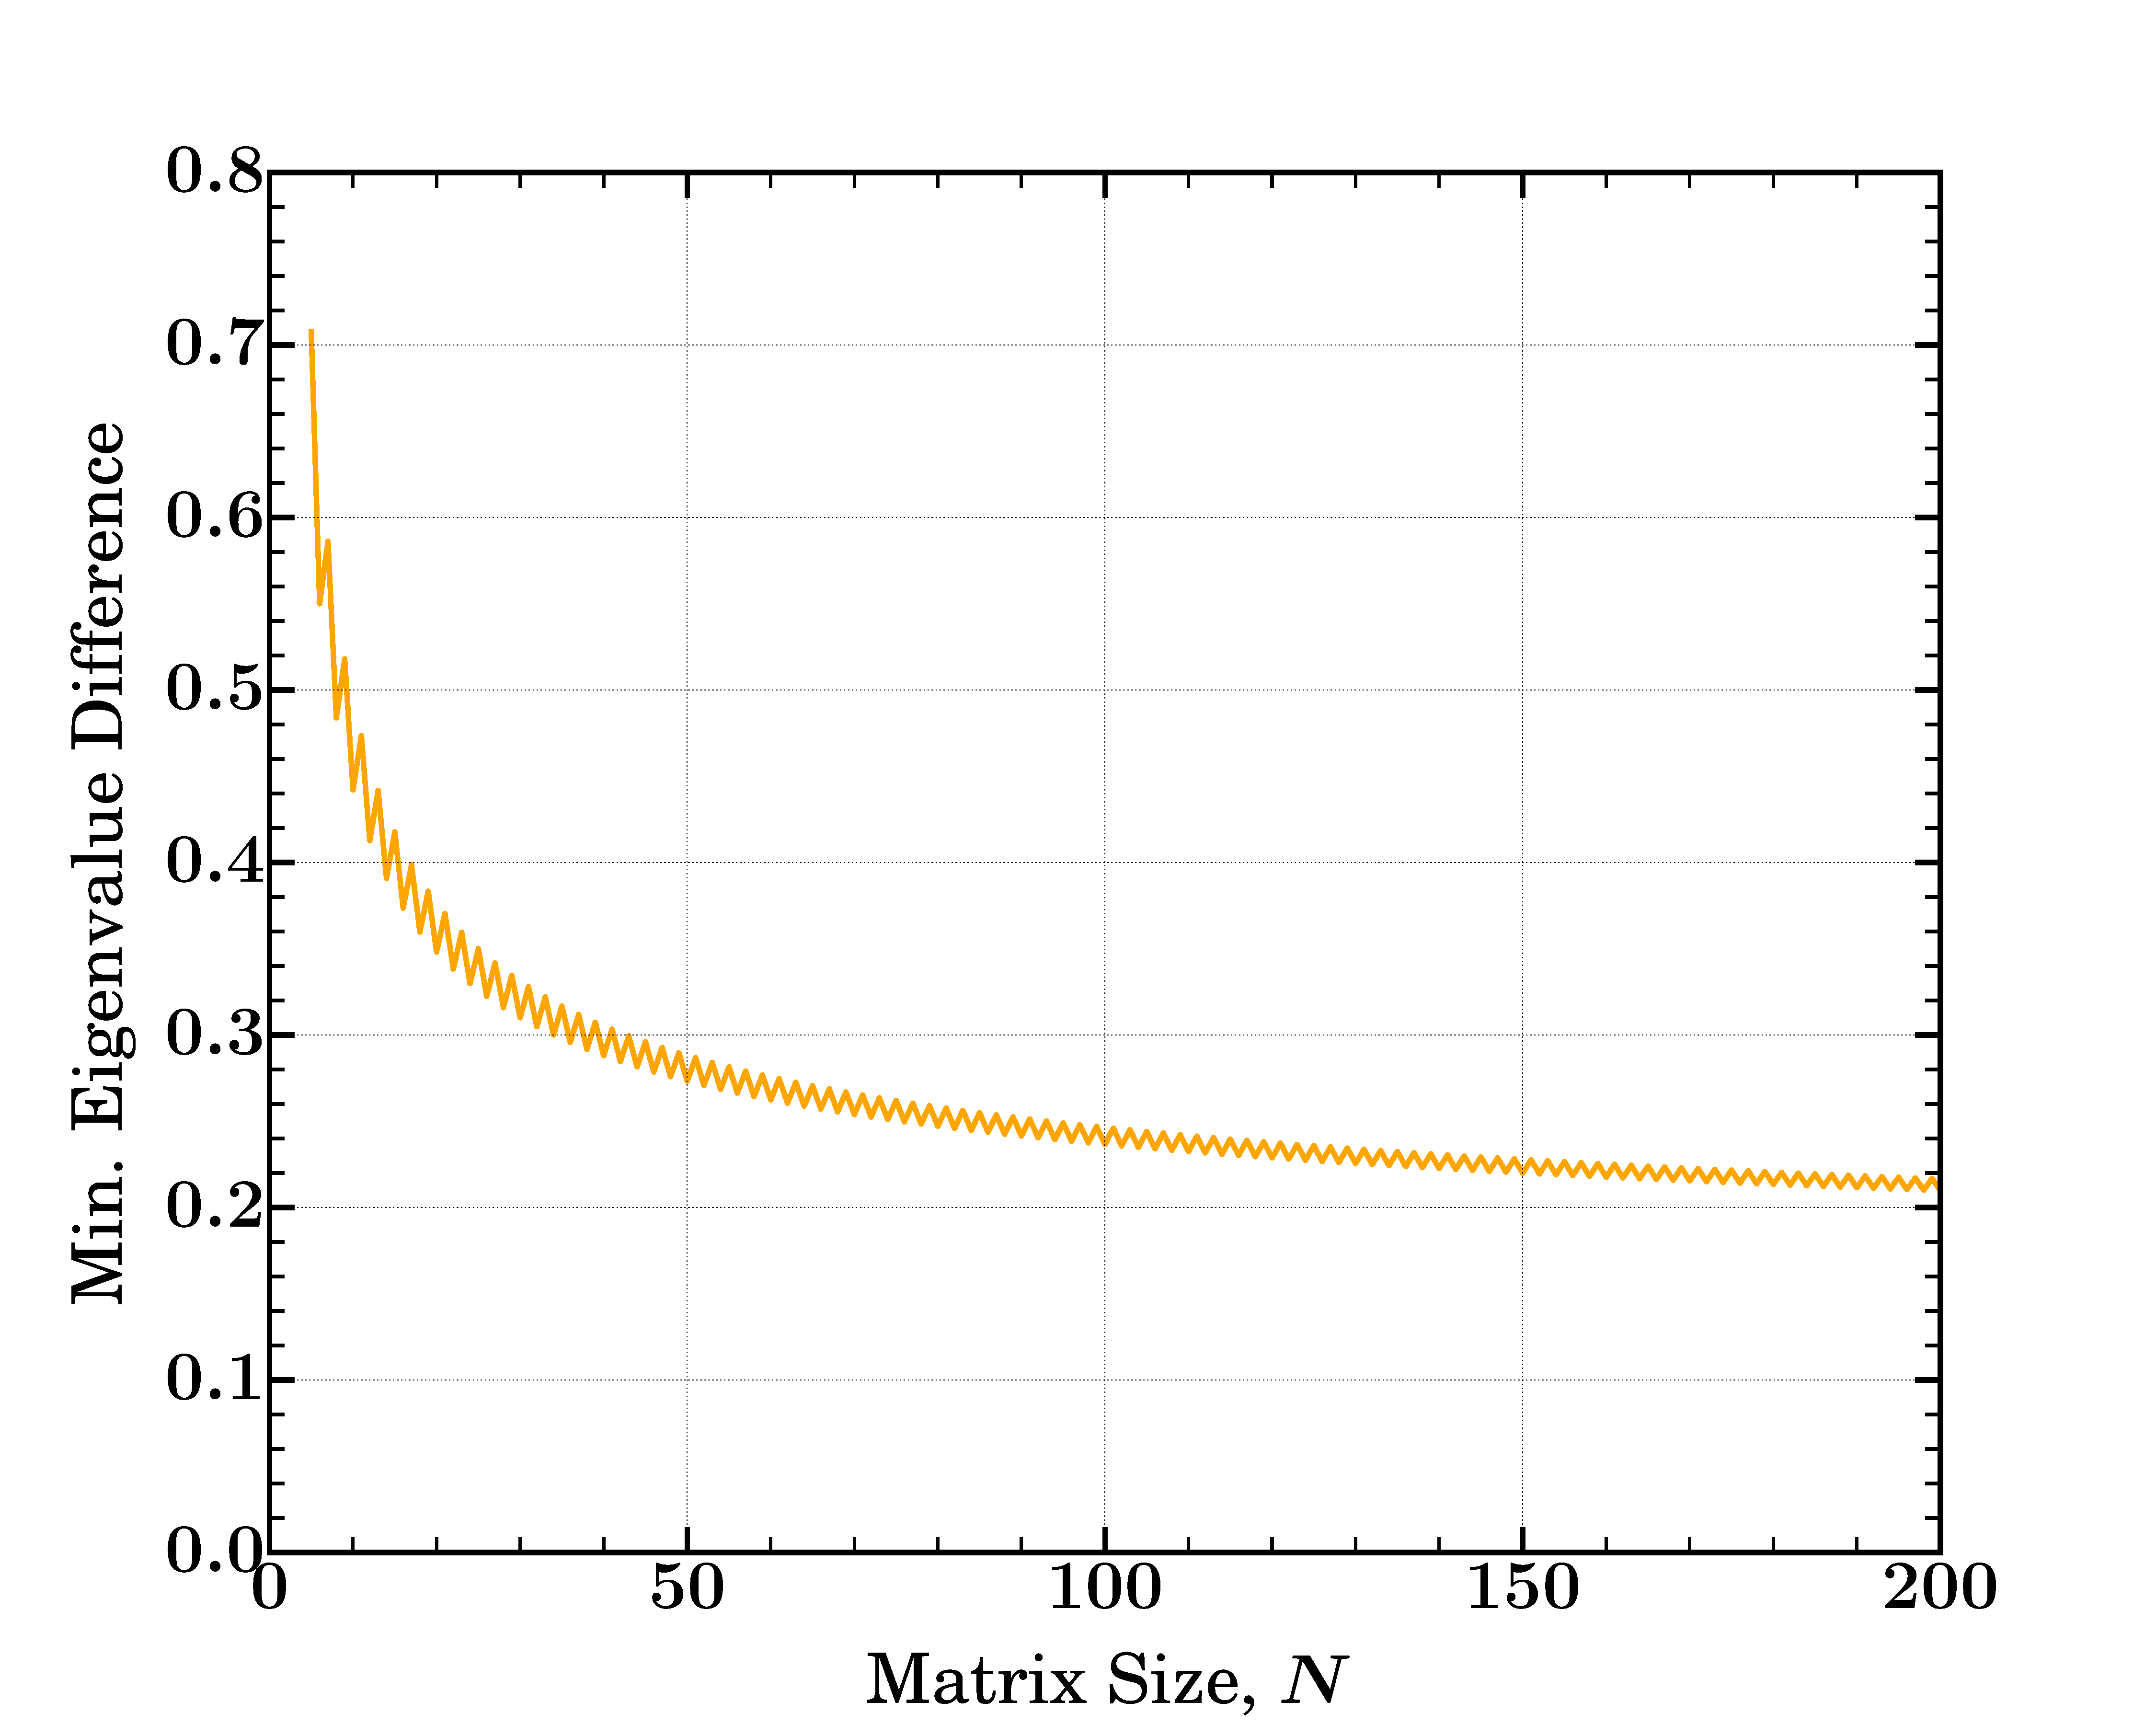
\includegraphics[width=\columnwidth]{figures/qm_min_eigenvalues_differences.pdf}
\caption{A plot of how the minimum successive eigenvalue difference (minimum level spacing) varies with the size of the matrix we choose to represent our Hamiltonian $H$. }
\label{fig:qm_min_eigenvalues_differences}
\end{figure}

Figure \ref{fig:qm_min_eigenvalues_differences} shows a plot of how the minimum successive eigenvalue difference (minimum level spacing) varies with the size of the matrix we choose to represent our Hamiltonian $H$. Two immediately interesting things can be noticed here. First, there seems to be a very well-defined, very specific way in which the minimum difference (which corresponds to the left-cuttoff in Figure \ref{fig:everything}) varies with $N$. Second, that variation seems to be dependent on the parity of $N$. In particular, for odd values of $N$, the minimum difference seems to be larger than for what would otherwise be defined by whatever larger-scale model is applicable.

\begin{figure}
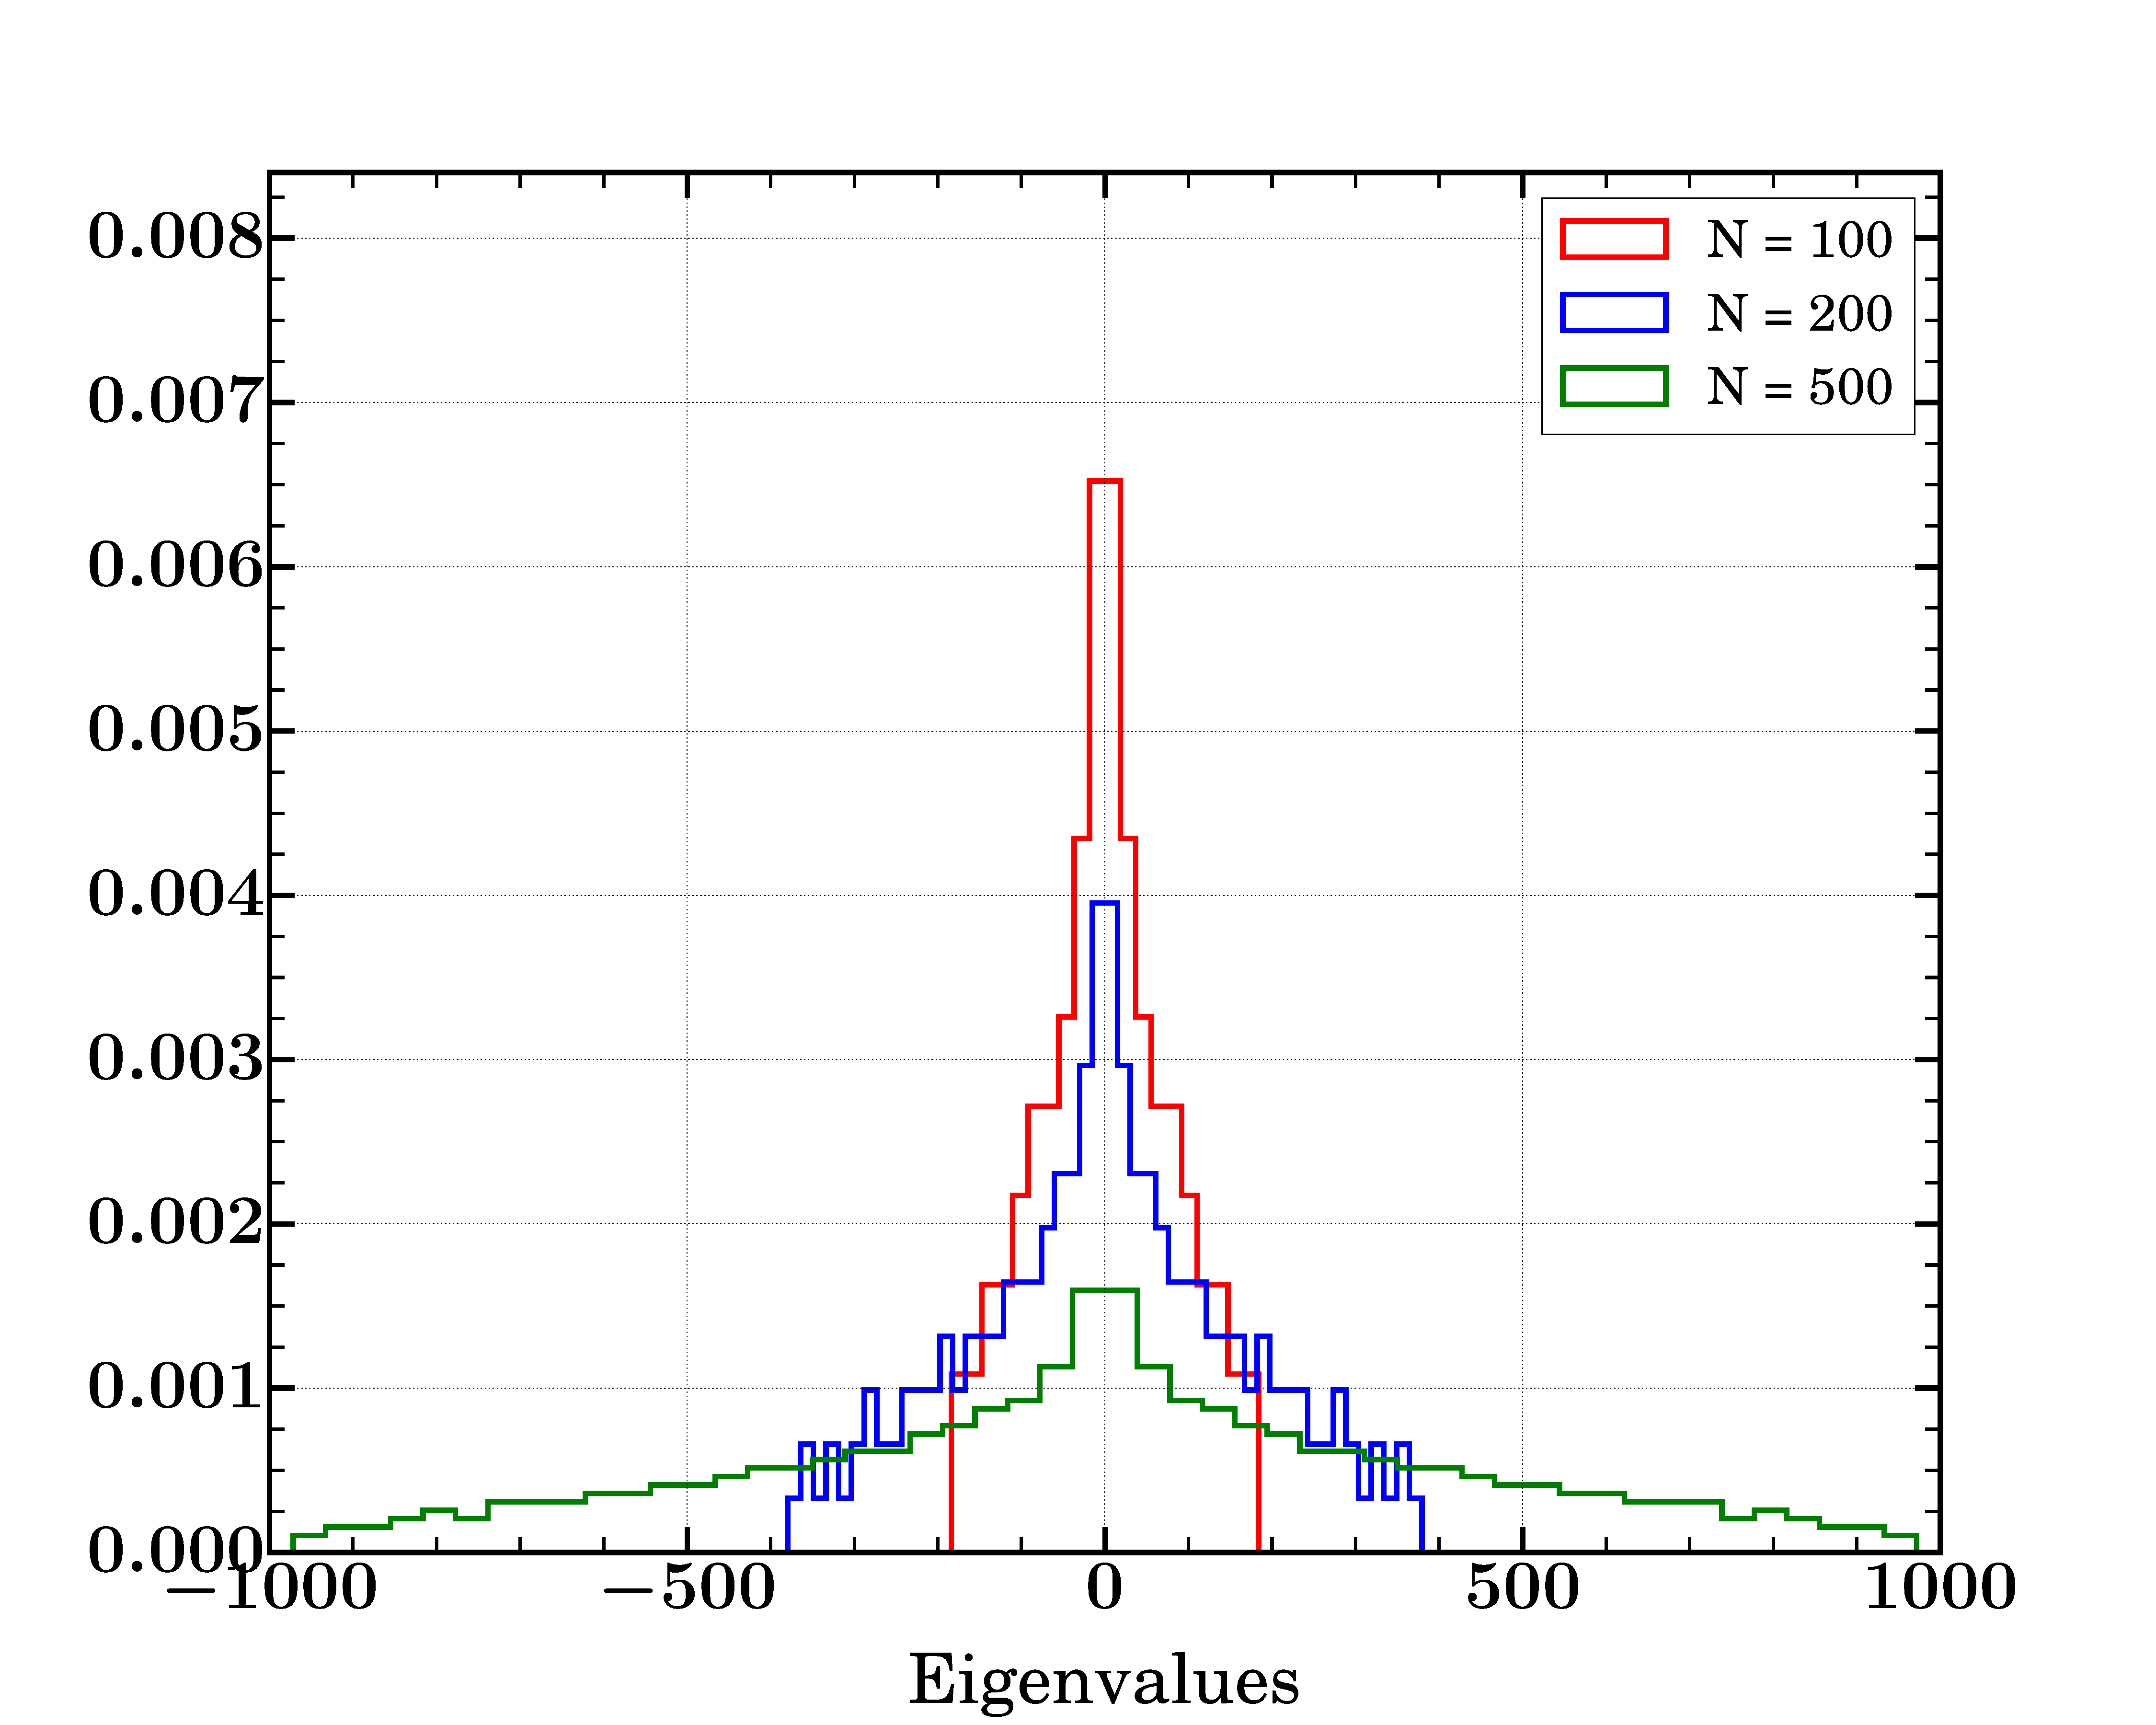
\includegraphics[width=\columnwidth]{figures/qm_eigenvalues.pdf}
\caption{A plot of how the minimum successive eigenvalue difference (minimum level spacing) varies with the size of the matrix we choose to represent our Hamiltonian $H$. }
\label{fig:qm_eigenvalues}
\end{figure}

Figure \ref{fig:qm_eigenvalues} shows a histogram of eigenvalues for a given $N \times N$ representation of $H$. The property we're particularly interested in is that the eigenvalues seem to be clustered around the origin. So, we conjecture, without proof, that the minimum eigenvalue difference is always going to be the difference of the two eigenvalues closest to the origin. 

However, there is a slight technicality here. For odd values of $N$, the matrix representation of $H$ is not invertible. In particular, it's rank is always going to be $N - 1$, which means it will have at most $N - 1$ non-zero eigenvalues. Said in other words, there will be one or more $0$ eigenvalues for odd $N$. However, if there were more than one $0$ eigenvalues, the minimum eigenvalue difference would be $0$, which doesn't seem to be the case for finite $N$ according to Figure \ref{fig:qm_min_eigenvalues_differences}. This means, for odd $N$'s, there will always be one zero eigenvalue. 

Because our matrix representation of $H$ only contains real entries, all its eigenvalues will occur as complex-conjugate pairs. These get divided by the $i$ factor outside to give real eigenvalues but this means that the eigenvalues will be symmetric about the origin, the only difference between odd and even $N$ being whether or not $0$ is one of those eigenvalues. 

\begin{figure}
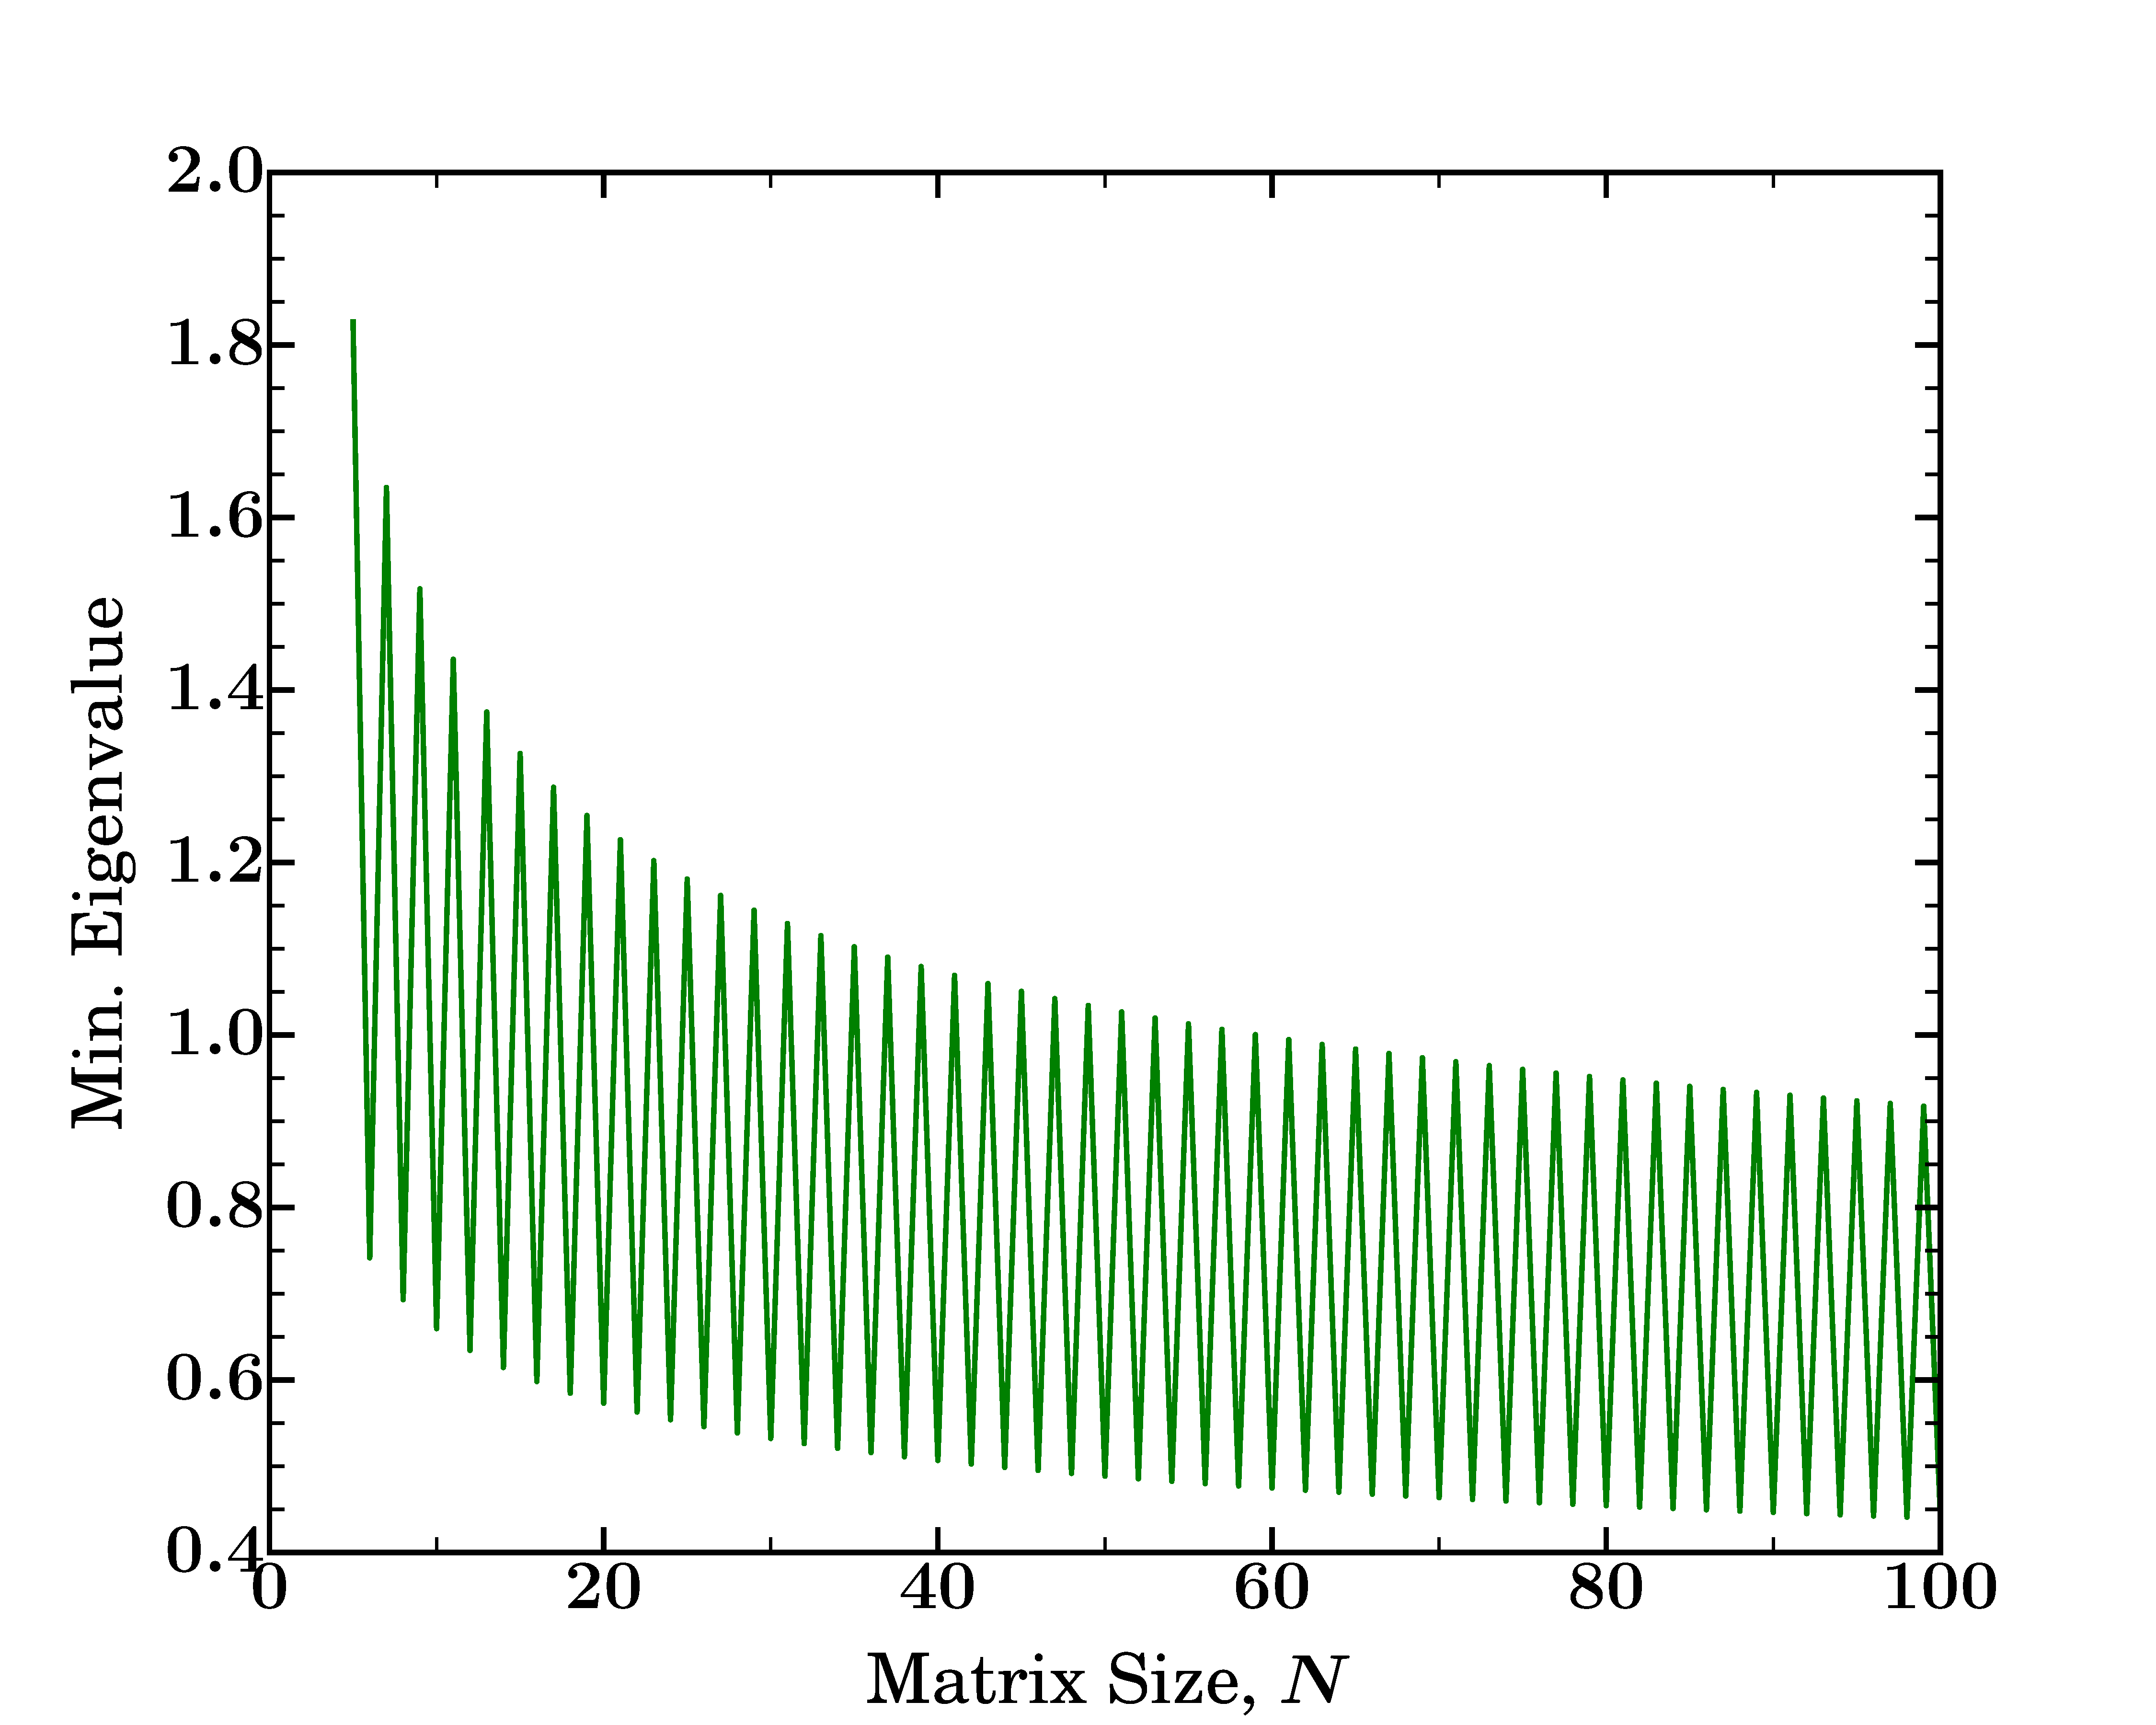
\includegraphics[width=\columnwidth]{figures/qm_min_eigenvalues.pdf}
\caption{A plot of how the minimum eigenvalues $\lambda_{+1}$ varies with the size of the matrix we choose to represent our Hamiltonian $H$. Note that for odd $N's$, the minimum would be $0$, so we choose the next largest minimum. In other words, we're plotting the minumum non-zero eigenvalues of $H$ against the size of its matrix representation $N$. }
\label{fig:qm_min_eigenvalues}
\end{figure}

For odd $N$'s, since we always have a $0$ eigenvalue, the min. difference would be just $\left| \lambda_{+1}^{\mathrm{odd}N} - \lambda_0^{\mathrm{odd}N} \right| = \left| \lambda_{+1}^{\mathrm{odd}N} - 0 \right| = \lambda_{+1}^{\mathrm{odd}N} $. However, for even values of $N$, since there is no zero eigenvalue, the minimum difference will be $\left| \lambda_{+1}^{\mathrm{even}N} - \lambda_{-1}^{\mathrm{even}N} \right| = \left|2 \lambda_{+1}^{\mathrm{even}N} \right| = 2 \lambda_{+1}^{\mathrm{even}N} $. Naively, it'd seem that therefore the minimum difference for even $N$'s would be larger than for odd $N$'s. However, as suggested by Figure \ref{fig:qm_min_eigenvalues_differences}, this is not true. It's important to note that $\lambda_{+1}^{\mathrm{even}N} \ne \lambda_{+1}^{\mathrm{odd}N}$, and so our argument breaks down. In fact, because the minimum  difference for odd $N$'s seems to always be larger than for even $N$'s, we can say that $ 2 \lambda_{+1}^{\mathrm{even}N} < \lambda_{+1}^{\mathrm{odd}N}$. Of course, this relation is not exactly well defined since $N$ will either be odd or will be even so there isn't a proper way to compare $\lambda_{+1}$ since the matrix size changes. So an implicit assumption in the relation is, ``what would normally be defined by the broader large-scale model''. Figure \ref{fig:qm_min_eigenvalues} demonstrates our claim.

Another important property of the plot in Figure \ref{fig:qm_min_eigenvalues_differences} we're interested in is the asymptotic behavior of the difference as $N \to \infty$. Ultimately, our aim is to find a Hilbert-Polya Hamiltonian and that would have an infinite-dimensional matrix representation (with infinitely many real eigenvalues which correspond to the imaginary parts of the infinitely many non-trivial roots of $\zeta(t)$) so, it's important to study the behavior of the matrix representation of $H$ as $N \to \infty$.

From Figure \ref{fig:qm_min_eigenvalues_differences}, it's not quite clear whether the difference approaches 0 or some finite value (that's very close to $0$) as $N \to \infty$. We conjecture that it does approach $0$. Here's a non-rigorous, hand-wavy reasoning. As seen in Figure \ref{fig:qm_eigenvalues}, the eigenvalues are symmetric about the origin. So when we compute the successive differences, consider approaching it from left and right i.e. moving from the most positive eigenvalue in the direction of decreasing eigenvalues and at the same time, moving from the most negative eigenvalue towards decreasingly negative eigenvalues. Because of the inherent symmetry in the eigenvalues, we must approach the same limiting value. However, if this limit positive, that would mean that we'd have to hit $0$ and move towards positive differences. But all the eigenvalues to the left of $0$ are negative so the differences can never be positive. Same with while moving from right to left, the differences can never be negative. But, since we have to approach the same limiting value for either case, this limit must be $0$.

But if the eigenvalue difference does hit $0$ when $H$ is infinite-dimensional, that would mean there is a degeneracy. However, because the eigenvalues of $H$ would correspond to the imaginary parts of the non-trivial roots of $\zeta(t)$ and so a degeneracy in the eigenvalues of $H$ implies a degeneracy in the non-trivial roots of $\zeta(t)$. Since no such degeneracy is known, any quantization of $H$ that would be a prospective Hilbert-Polya Hamiltonian would have to have something to break this degeneracy. Note that even though it seems like the difference in roots of $\zeta(t)$ in Figure \ref{fig:everything} seems to be going all the way down to 0, it does not. For the plot produced, which contains the first 2 million zeros, it goes all the way down to $\sim 0.0052$ (in normalized units). 

\section{Conclusion}
So this is the conclusion. Haha

%    Ordinary theorem and proof
%\begin{theorem}[Optional addition to theorem head]
% text of theorem
%\end{theorem}

%\begin{proof}[Optional replacement proof heading]
% text of proof
%\end{proof}

%    Figure insertion; default placement is top; if the figure occupies
%    more than 75% of a page, the [p] option should be specified.
%\begin{figure}
%\includegraphics{filename}
%\caption{text of caption}
%\label{}
%\end{figure}


%    Text of article.

%    Bibliographies can be prepared with BibTeX using amsplain,
%    amsalpha, or (for "historical" overviews) natbib style.
\bibliographystyle{amsplain}
%    Insert the bibliography data here.

\end{document}

%-----------------------------------------------------------------------
% End of article-template.tex
%-----------------------------------------------------------------------